% REMEMBER: You must not plagiarise anything in your report. Be extremely careful.

\documentclass{l4proj}

    
%
% put any additional packages here
%

\begin{document}

%==============================================================================
%% METADATA
\title{HarmonyScape: Inclusive 3D Exploration with Music for those living with Dementia}
\author{Robbie Tippen}
\date{March 22, 2024}

\maketitle

%==============================================================================
%% ABSTRACT
\begin{abstract}
    
    This dissertation investigates the development and implementation of HarmonyScape, an inclusive initiative tailored for individuals with intellectual disabilities, including Alzheimer's. Inspired by the profound link between music and cognitive function, HarmonyScape creates a captivating 3D world where music dynamically responds to user exploration. Through character control in an open-world setting and interactive music-based mini games, players unlock new instruments, filling out the games' musical landscape. The project's aim is to provide a multi-sensory environment that potentially aids cognitive well-being while offering an engaging, interactive experience. Initial user feedback indicates high levels of engagement and enjoyment, suggesting promising avenues for inclusive gaming and therapeutic interventions. This research underscores the significance of tailored approaches to accessibility and engagement in fostering cognitive well-being among individuals with intellectual disabilities.
    \vskip 0.5em
    Every abstract follows a similar pattern. Motivate; set aims; describe work; explain results.
    \vskip 0.5em
    ``XYZ is bad. This project investigated ABC to determine if it was better. 
    ABC used XXX and YYY to implement ZZZ. This is particularly interesting as XXX and YYY have
    never been used together. It was found that  
    ABC was 20\% better than XYZ, though it caused rabies in half of subjects.''
\end{abstract}

\begin{abstract}
    \textbf{Inclusive 3D Exploration with Music for Intellectual Disabilities}

 

    Imagine an inclusive initiative tailored specifically for individuals with intellectual disabilities, including conditions like Alzheimer's. Through Unity, we plan to create a captivating 3D world that generates music in response to exploration. This project is inspired by the unique relationship between music and cognitive function (Baird \& Samson, 2015), and its therapeutic potential for those with dementia (Vink et al., 2003). By immersing users in a visually engaging environment where music dynamically responds to movement, we aim to provide a multisensory experience that not only captivates but also potentially aids cognitive well-being in an enjoyable, interactive manner.

 

    \textbf{Reading}  
    
    Baird, A., \& Samson, S. (2015). Music and dementia. Progress in brain research, 217, 207-235.
    
     
    
    Vink, A. C., Bruinsma, M. S., \& Scholten, R. J. (2003). Music therapy for people with dementia. Cochrane database of systematic reviews, (4).
\end{abstract}

%==============================================================================

% EDUCATION REUSE CONSENT FORM
% If you consent to your project being shown to future students for educational purposes
% then insert your name and the date below to  sign the education use form that appears in the front of the document. 
% You must explicitly give consent if you wish to do so.
% If you sign, your project may be included in the Hall of Fame if it scores particularly highly.
%
% Please note that you are under no obligation to sign 
% this declaration, but doing so would help future students.
%
\def\consentname {Robbie Tippen} % your full name
\def\consentdate {27 February 2024} % the date you agree
%
\educationalconsent


%==============================================================================
\tableofcontents

%==============================================================================
%% Notes on formatting
%==============================================================================
% The first page, abstract and table of contents are numbered using Roman numerals and are not
% included in the page count. 
%
% From now on pages are numbered
% using Arabic numerals. Therefore, immediately after the first call to \chapter we need the call
% \pagenumbering{arabic} and this should be called once only in the document. 
%
% Do not alter the bibliography style.
%
% The first Chapter should then be on page 1. You are allowed 40 pages for a 40 credit project and 30 pages for a 
% 20 credit report. This includes everything numbered in Arabic numerals (excluding front matter) up
% to but excluding the appendices and bibliography.
%
% You must not alter text size (it is currently 10pt) or alter margins or spacing.
%
%
%==================================================================================================================================
%
% IMPORTANT
% The chapter headings here are **suggestions**. You don't have to follow this model if
% it doesn't fit your project. Every project should have an introduction and conclusion,
% however. 
%
%==================================================================================================================================
\chapter{Introduction}

% reset page numbering. Don't remove this!
\pagenumbering{arabic} 

% The project is inspired by research indicating the therapeutic potential of music for individuals with dementia, as highlighted by studies such as Vink et al. (2003). By leveraging the relationship between music and cognitive function, the initiative seeks to explore how interactive music experiences can benefit individuals with intellectual disabilities.

TOODO: \begin{itemize}
    \item Abstract
    \item Present continuous tense (Happened already and continue happening)
    \item Fix use of singular and double quotation marks
    \item Should have objectives (more than 1 or 2 that are more specific, and act as stepping stones to reach the aims)
    \item Should only have 1 or 2 aims (not as specific)
\end{itemize}


This opening chapter sets the stage for the HarmonyScape project by introducing the motivations and goals that led to its development. The following sections of this paper will explore distinct segments of the project, covering its background, design, implementation, and evaluation.

\section{Motivation}
As the prevalence of dementia increases within our aging population, with the number of older people with dementia in the UK projected to rise by 80\% from almost 885,000 in 2019 to around 1.6 million in 2040 (Wittenberg \emp{et al.,} 2019), the development of effective treatments and engaging activities to manage its symptoms becomes imperative.  The means of music as a form of therapy in the treatment of diseases linked with dementia, such as Alzheimer's, is a unique approach that taps into preserved cognitive and emotional functions in individuals with dementia.

Research by Vink AC \emph{et al.} (2004) shows promising results that for individuals with dementia, music-based therapeutic interventions can be employed to target depressive symptoms. While the potential benefits of game-based activities for cognitive function in dementia are highlighted by Vilkki et al. (2019), combining these approaches in a therapeutic setting has been seldom explored. This suggests a valuable avenue for future research in dementia care.

This combined approach is particularly promising for our aging population. As lifespans increase, so does the prevalence of dementia. However, this generation also coincides with a rise in video game popularity. People who were 14 years old in 1973, the year the first home video game console, the Magnavox Odyssey\footnote{https://www.computinghistory.org.uk/det/16909/Magnavox-Odyssey/}, was released globally, would be 65 today. This being the age where the risk of dementia significantly increases (Chen \emph{et al.,} 2009). This generation's familiarity with games can be leveraged to create engaging and effective therapeutic activities. Despite the clear potential of this promising avenue for leveraging a familiar and potentially engaging activity, it remains largely unexplored.

% - multisensory experiences provide mental and emotional stimulation for those with alzhiemers

- enjoyment of music is something that doesn't dissipate as dementia progresses

\section{Aims}
Considering the motivations outlined above, we will develop a multisensory, interactive 3D exploration game designed to potentially aid cognitive well-being in those with dementia, including diseases like Alzheimer's. This game will prioritise enjoyment and captivation while incorporating active music theory principles, where the soundscape dynamically responds to player movement.

An evaluation will then be conducted to address the following question:
Is the project a means of captivating and potentially aiding cognitive well-being in an enjoyable, interactive manner?

This is a broad and complex question that cannot be definitively answered in a single evaluation, especially at this scale. Thus, we present four key questions to help answer the broader question

\begin{itemize}
    \item How intrinsically motivating is the game? Does the multisensory design and interactive music system encourage engagement from the player?
    \item How pleasant and satisfying is the dynamic music-making system for players? Does it promote a sense of creative control and enjoyment?
    \item Does the game show potential for aiding cognitive well-being in individuals with dementia?
    \item Does the game induce any negative effects, such as stress or confusion, which could affect players with dementia?
\end{itemize}

% Why should the reader care about what are you doing and what are you actually doing?
% \section{Guidance}

% \textbf{Motivate} first, then state the general problem clearly. 

% \section{Writing guidance}
% \subsection{Who is the reader?}

% This is the key question for any writing. Your reader:

% \begin{itemize}
%     \item
%     is a trained computer scientist: \emph{don't explain basics}.
%     \item
%     has limited time: \emph{keep on topic}.
%     \item
%     has no idea why anyone would want to do this: \emph{motivate clearly}
%     \item
%     might not know \emph{anything} about your project in particular:
%     \emph{explain your project}.
%     \item
%     but might know precise details and check them: \emph{be precise and
%     strive for accuracy.}
%     \item
%     doesn't know or care about you: \emph{personal discussions are
%     irrelevant}.
% \end{itemize}

% Remember, you will be marked by your supervisor and one or more members
% of staff. You might also have your project read by a prize-awarding
% committee or possibly a future employer. Bear that in mind.

% \subsection{References and style guides}
% There are many style guides on good English writing. You don't need to
% read these, but they will improve how you write.

% \begin{itemize}
%     \item
%     \emph{How to write a great research paper} \cite{Pey17} (\textbf{recommended}, even though you aren't writing a research paper)
%     \item
%     \emph{How to Write with Style} \cite{Von80}. Short and easy to read. Available online.
%     \item
%     \emph{Style: The Basics of Clarity and Grace} \cite{Wil09} A very popular modern English style guide.
%     \item
%     \emph{Politics and the English Language} \cite{Orw68}  A famous essay on effective, clear writing in English.
%     \item
%     \emph{The Elements of Style} \cite{StrWhi07} Outdated, and American, but a classic.
%     \item
%     \emph{The Sense of Style} \cite{Pin15} Excellent, though quite in-depth.
% \end{itemize}

% \subsubsection{Citation styles}

% \begin{itemize}
% \item If you are referring to a reference as a noun, then cite it as: ``\citet{Orw68} discusses the role of language in political thought.''
% \item If you are referring implicitly to references, use: ``There are many good books on writing \citep{Orw68, Wil09, Pin15}.''
% \end{itemize}

% There is a complete guide on good citation practice by Peter Coxhead available here: \url{http://www.cs.bham.ac.uk/~pxc/refs/index.html}. 
% If you are unsure about how to cite online sources, please see this guide: \url{https://student.unsw.edu.au/how-do-i-cite-electronic-sources}.

% \subsection{Plagiarism warning}

% \begin{highlight_title}{WARNING}
    
%     If you include material from other sources without full and correct attribution, you are commiting plagiarism. The penalties for plagiarism are severe.
%     Quote any included text and cite it correctly. Cite all images, figures, etc. clearly in the caption of the figure.
% \end{highlight_title}


%==================================================================================================================================
\chapter{Background}
To DO:
\begin{itemize}
    \item Beginning section
    \item Add to Dementia section that its more specifically aimed at those with early to mid stages of dementia and that’s what I’m referring to from here on out when referring to those living with dementia
    \item Definition of Gamification
\end{itemize}


\section{Dementia}

Throughout this dissertation, I will use the term 'dementia' as an umbrella term for diseases that cause the decline in cognitive abilities that impacts a person's ability to perform everyday activities, which typically involves problems with memory, thinking, and behavior.  Dementia is a progressive condition, meaning symptoms worsen over time. While there are many causes of dementia, the most common is Alzheimer's disease.

\subsection{Alzheimer's disease}
Alzheimer's disease is a progressive neurological disorder that can affect memory, thinking skills and behaviour. As of 2024, it is the most common cause of dementia, a group of brain disorders that result in loss of intellectual and social skills that is severe enough to interfere with daily functioning (Li et al., 2024). Alzheimer's typically begins slowly and as the disease progresses, individuals can experience memory loss, confusion, difficulty with language and communication, impaired judgment, and changes in personality (Li et al., 2024). Currently, there is no cure for Alzheimer's disease, but treatments and interventions can manage symptoms and improve quality of life for those affected by the disease.

Both pharmacological and non-pharmacological treatments have been trialed to alleviate symptoms of dementia. Pharmacological treatments, lik acetylcholinesterase inhibitors, primarily target cognitive symptoms without altering the progression of the disease. These treatments have shown minimal effectiveness in easing the behavioral and psychological symptoms linked to these diseases (Dyer et al., 2018).

Conversely, non-pharmacological interventions offer supplementary treatments, presenting diverse strategies to enhance the well-being of individuals with dementia, reduce behavioral incidents, and enhance or maintain their quality of life (Dyer et al., 2018).

\section{Music Therapy}\label{sec:music_therapy}

Music therapy is defined by the World Federation of Music Therapy (2011) as the professional application of musical elements (sound, rhythm, melody, and harmony) by qualified therapists to facilitate communication, relationships, learning, expression, and other therapeutic objectives. It is employed across medical, educational, and everyday settings to optimise quality of life and enhance physical, social, communicative, emotional, intellectual, and spiritual health and well-being.

\emph{Music therapy for people with dementia} by Vink AC \emph{et al.} (2004) discusses music therapy as one potential non-pharmacological treatment for people with different forms of dementia, such as Alzheimer's. Of particular relevance to our aims are the discussions of the distinct varieties of music therapy, Vink AC \emph{et al.} (2004) distinguish two main types of music therapy.
\newline

\textbf{Receptive Music Therapy}
\newline

In receptive music therapy, individuals passively engage with music chosen or performed by the therapist. They may listen to live music, recordings, or the therapist's singing. This form of therapy focuses on the emotional and psychological responses evoked by the music. The therapist selects music tailored to the individual's needs, aiming to stimulate relaxation, emotional expression, or cognitive engagement (Vink AC \emph{et al.} 2004).
\newline

\textbf{Active Music Therapy}
\newline

Active music therapy involves active participation from the individual receiving therapy. This can include playing musical instruments, singing, improvisation, or engaging in structured music activities led by the therapist. Active participation encourages physical movement, cognitive stimulation, social interaction, and self-expression. It empowers individuals to actively engage with music-making processes, fostering a sense of agency and creativity in a therapeutic environment (Vink AC \emph{et al.} 2004).


\section{Dementia and Cognitive Stimulation}
This section explores the impact of dementia on cognitive function, and introduces strategies for cognitive stimulation, including traditional games, spatial puzzles, and interventions targeting attention and neuroplasticity.

\subsection{Familiarity and Engagement in Traditional Games}\label{sec:traditional_games}
De Siqueira et al. (2017) discusses the advantages of utilising well-known traditional games in the development of games tailored for individuals with intellectual disabilities like Alzheimer's. Since many elderly individuals are likely familiar with the rules of these games, minimal introduction and assistance are required for them to be engaged (De Siqueira et al., 2017). Moreover, for those with Alzheimer's, playing these games can evoke memories of past experiences, such as playing as children or with grandchildren, thus facilitating a personalised approach that enhances engagement and motivation (De Siqueira et al., 2017). By incorporating personalisation, memory training games can be even more effective for Alzheimer's patients (Eichhorn et al., 2018).


\subsection{Traditional Sliding Puzzles in the Treatment of Dementia}\label{sec:sliding_dementia}

Sasaki et al. (2020) explored the use of sliding puzzle's in the treatment of dementia with their brain training application. This is where the user manipulates the panel within a single frame, utilising available space to organise it according to the desired arrangement (Sasaki et al., 2020). The act of sliding the puzzle pieces activates the frontal lobe, responsible for memory, as the user anticipates the direction in which the moving panels can be adjusted to achieve the desired order (Hirono et al., 1997). The user is required to alter the positions of the panels within the sliding block puzzle while retaining the original layout in memory (Sasaki et al., 2020).

The spatial recognition capacity of the frontal lobe is engaged as the user formulates the steps necessary to reach the correct solution by comprehending the panel positions (Hirono et al., 1997). Completing the puzzle requires players to retain memory, arrange figures, and comprehend spatial relationships. This combination of cognitive skills may have the potential to slow dementia progression, as suggested by research from Sasaki et al. (2020).


\subsection{Attention impairments}\label{sec:attention}
Attention impairments in Alzheimer’s Disease represent a significant aspect of the cognitive decline observed in affected individuals, despite Alzheimer’s Disease being primarily recognized as a memory disorder (Hennawy et al., 2019).

\subsubsection{Selective Attention}
pertains to the cognitive capacity to focus on a singular stimulus while ignoring surrounding distractions (Chau et al., 2015). Impairments in selective attention exacerbate linearly with Alzheimer’s Disease severity (Chau et al., 2015).

\subsubsection{Sustained Attention} is differentiated from other classes of attention by the duration of the required activity (Fortenbaugh et al., 2017). More specifically, sustained attention is defined as the capacity to sustain focus on a particular task over an extended duration (Fortenbaugh et al., 2017).

\subsection{Neuroplasticity}\label{sec:neuroplasticity}
Neuroplasticity refers to the brain's ability to adapt and modify its structure and function throughout life (Costandi, 2016). This includes the formation of new neural connections, the strengthening of existing ones, and even rewiring itself in response to experiences and learning (Costandi, 2016). For people living with dementia, this process is disrupted, leading to the degeneration of brain cells and connections, ultimately causing cognitive decline (Koch and Spampinato, 2022).

Research by Hill, Kolanowski, and Gill (2011) has shown that utilising remaining brain plasticity is a promising avenue for potentially slowing down the progression of dementia. This residual neuroplasticity offers a window of opportunity for non-pharmacological interventions designed to stimulate cognitive function, which can improve spatial awareness and memory in those with dementia(Boggio et al., 2011).

\subsection{Auditory and Spatial Games}
One promising means for utilising neuroplasticity is through games specifically designed to challenge auditory processing and spatial awareness. These games can provide a stimulating environment that promotes:

\subsubsection{Formation of new neural connections:} By engaging in novel tasks that challenge auditory processing and spatial reasoning, the brain is encouraged to form new connections between neurons (Park and Bischof, 2013). This strengthens communication within existing networks and can potentially create new pathways for cognitive function (Park and Bischof, 2013).

\subsubsection{Strengthening existing connections:} Park and Bischof (2013) also discuss how repeatedly playing these games can reinforce the neural connections used for processing sounds and navigating spatial environments. This reinforcement, as they explain helps maintain the health and efficiency of these connections, potentially slowing their decline in dementia.

\subsubsection{Improved cognitive function in key areas:} Studies by Boggio et al. (2011) suggest that stimulating cognitive function can improve spatial awareness and memory in dementia patients. Games that target these areas directly can provide targeted training and potentially enhance these critical cognitive skills (Park and Bischof, 2013).

\subsection{Noise Sensitivity in Dementia}\label{sec:noise_sensitivity}
Research by Shirsat, Jha and Verma (2023) highlights the negative effects that disruptive or unpleasant sounds can have on people living with dementia. Due to cognitive decline, dementia compromises the brain's ability to process and filter stimuli, making patients more sensitive to their surroundings (Shirsat, Jha and Verma, 2023). This means that noises others might easily ignore can cause confusion and agitation for those with dementia.

Sudden, loud, or jarring noises are especially likely to trigger a negative response, disrupting concentration, increasing anxiety, and contributing to behavioural problems (Shirsat, Jha and Verma, 2023). Even background noise can become overwhelming and disorienting for someone with dementia if it includes loud or jarring noises (Shirsat, Jha and Verma, 2023).

Understanding this impact is crucial in making HarmonyScape a supportive tool for individuals living with dementia. Minimising unnecessary noise, designing spaces with good acoustics, and using soothing sounds like calming music will be essential for promoting comfort and reducing distress for individuals with dementia as they explore the game (Caspar et al., 2017).

\subsection{Progress Tracking in Supporting Players with Dementia}\label{sec:progress_tracking}
Players with dementia often experience short-term memory challenges, making it difficult to recall previous actions or retain  information within a gameplay session. A progress tracker can be particularly helpful for this group, as it provides a visual and tangible representation of their achievements. Studies suggest that external memory aids, such as visual representations of progress, can support memory function in individuals with dementia (Bourgeois et al., 2003). Seeing progress reinforces a sense of accomplishment and  provides a clear marker of progress within the game. This, in turn, could enhance motivation and engagement for players living with dementia as they progress through HarmonyScape, potentially leading to improved well-being (Orrell et al., 2017). Furthermore, gamification elements like progress trackers can tap into this concept of positive reinforcement, promoting enjoyment within computerized activities (Vermeir et al., 2020).

\subsection{Third-Person Perspective in Dementia-Focused Game Design}\label{sec:third_person}
There are a cpuple of compelling reasons to consider a third-person perspective in games designed for those with dementia

Firstly, simulation sickness, a form of motion sickness induced by virtual environments, is a common issue in gaming, particularly within first-person perspectives (Hancock et al., 2008). This mismatch between visual cues of movement and a lack of corresponding physical motion can lead to nausea, disorientation, and headaches (Hancock et al., 2008). Individuals with cognitive decline may be especially susceptible to simulation sickness due to a decline in spatial awareness (Li et al., 2024). This difficulty in understanding their position in relation to the virtual environment can exacerbate feelings of disorientation, dizziness, and nausea that are common with simulation sickness (Lin et al., 2002). A study by Lin et al. (2002) demonstrated that a third-person perspective offers a potential solution, with individuals experiencing significantly fewer symptoms of simulator sickness when navigating a virtual environment from this viewpoint. By creating visual distance between the player and the character's movement, a third-person perspective lessens the sensory conflict that contributes to simulation sickness (Lin et al., 2002).

Secondly, a third-person perspective in video games significantly enhances situational awareness. This expanded viewpoint offers a greater field of view, enabling the player to simultaneously observe their character and a larger portion of the virtual environment (Denisova \& Cairns, 2015). This increased visual overview could be helpful in mitigating spatial disorientation and confusion (Denisova \& Cairns, 2015), which are common challenges in those with dementia (Li et al., 2024). The ability to see the player-controlled character within the context of the game world may provide a more stable reference point (Denisova \& Cairns, 2015), potentially aiding spatial understanding and awareness within the game.


\section{Related Works}
In my comprehensive review of existing literature, I found a notable absence of multisensory experiences tailored for individuals with intellectual disabilities such as Alzheimer’s that incorporate active music theory within a gaming setting. However, a range of experiences created for both academic and commercial purposes have been introduced with a similar goal as that of HarmonyScape in aiding those with intellectual disabilities, including conditions like Alzheimer’s, in enhancing their cognitive well-being in an enjoyable, interactive manner.

\subsection{AARP Staying Sharp}
AARP Staying Sharp is an online platform provided by AARP (formerly known as the American Association of Retired Persons) that offers a variety of brain-training games and activities designed to help individuals maintain cognitive function and mental acuity as they age. These games cover a range of cognitive skills such as memory, attention, problem-solving, and language.

\begin{figure}[h]
    \centering
    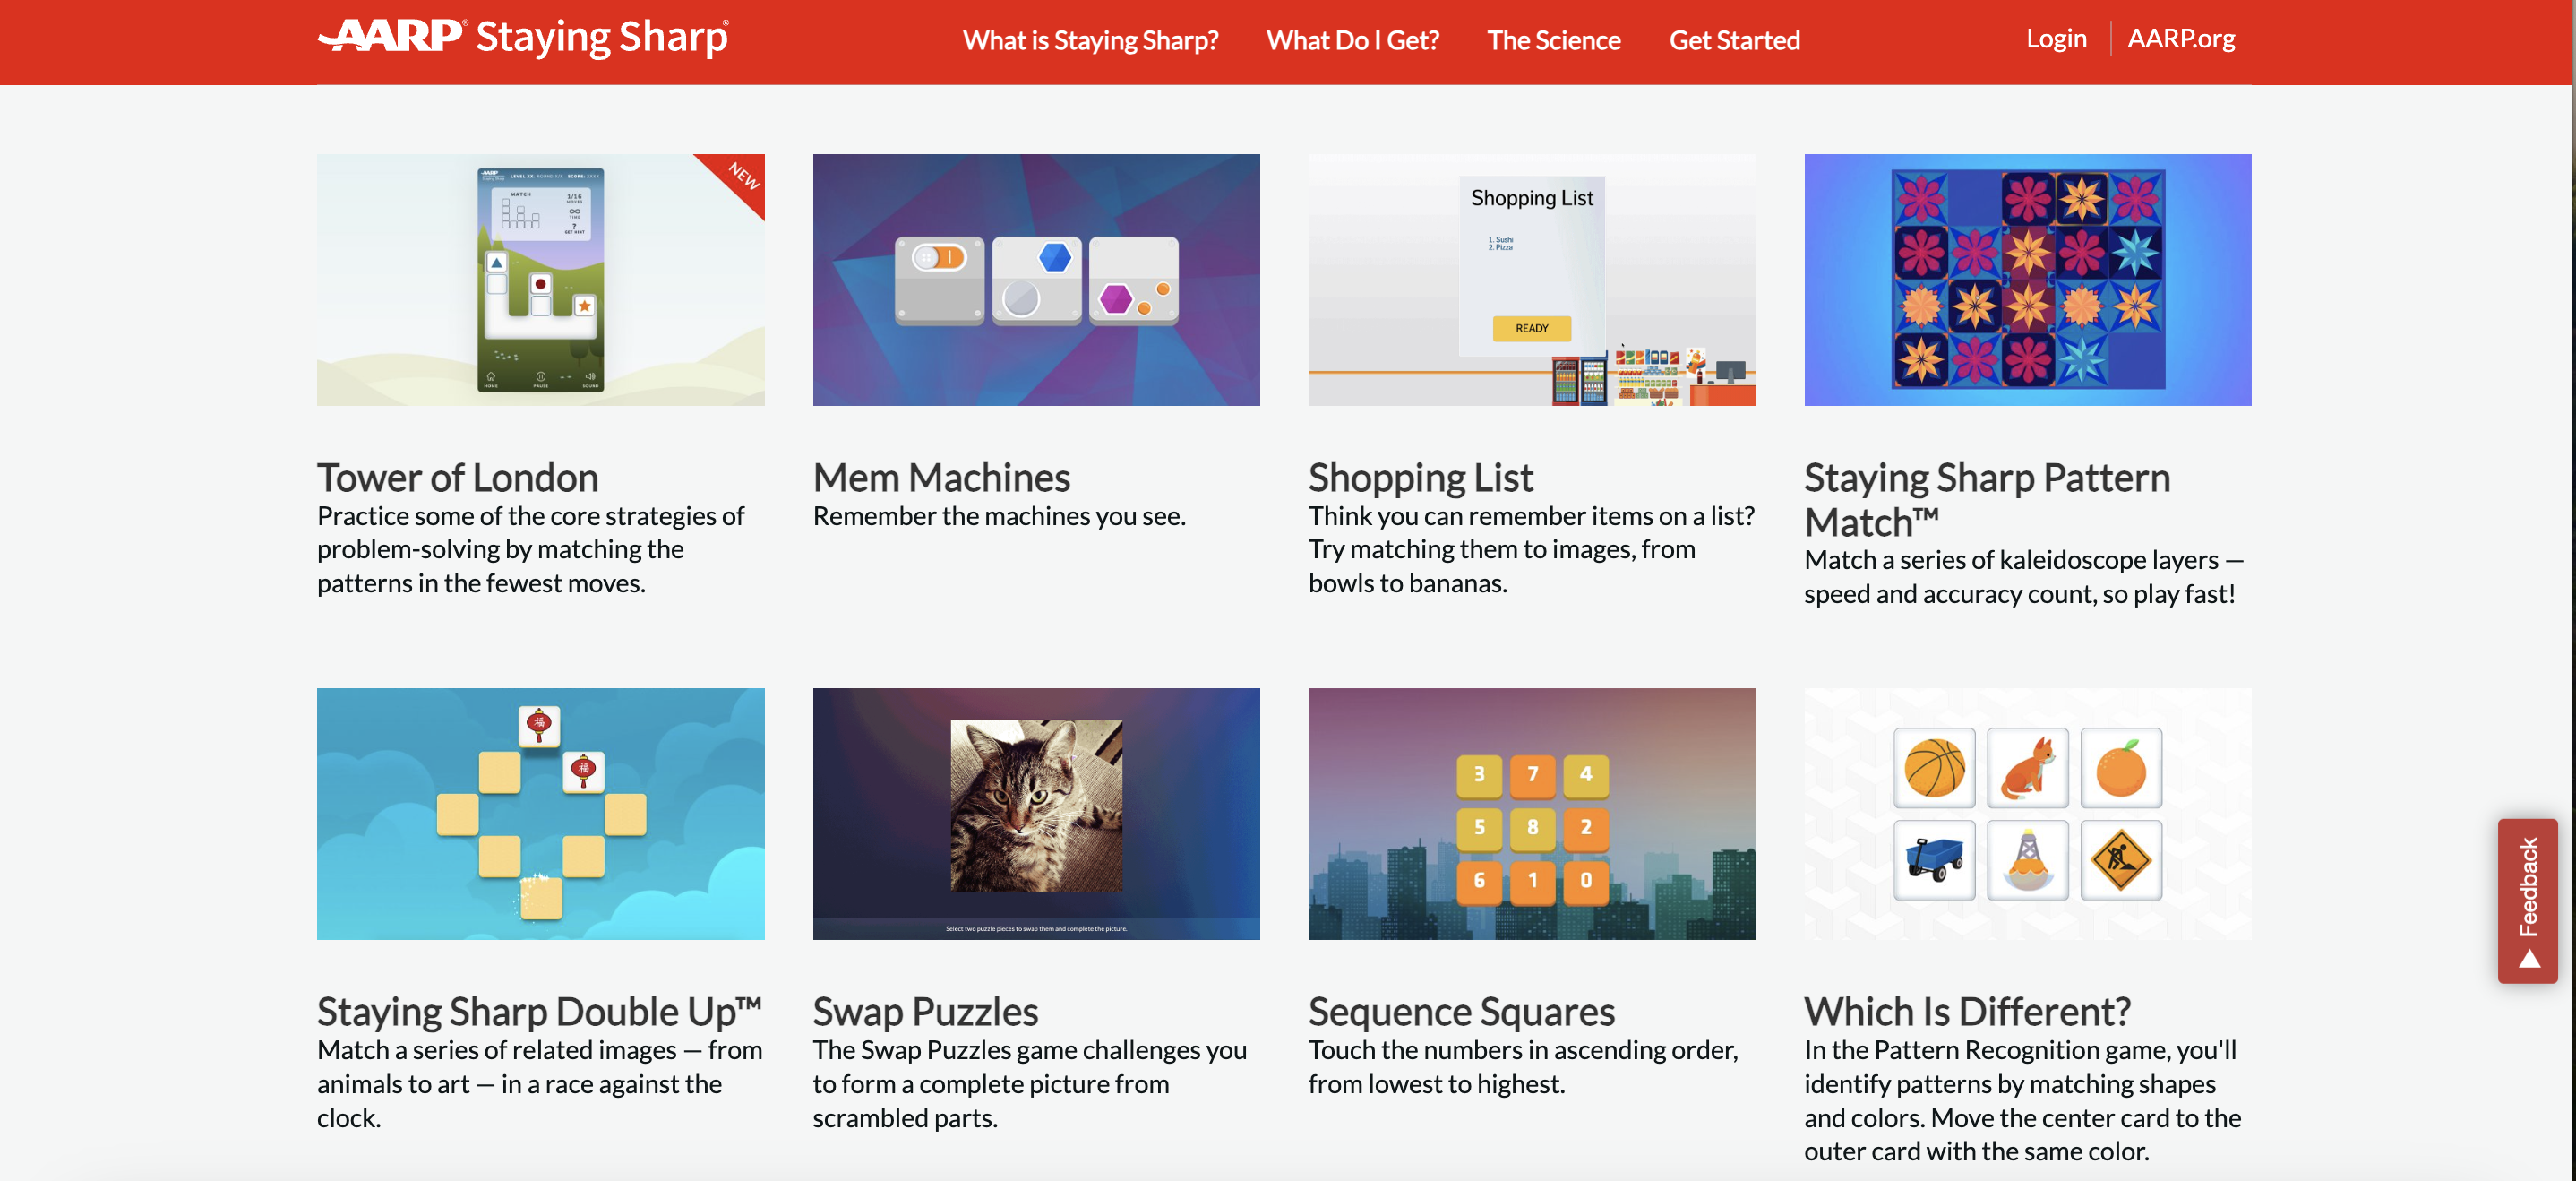
\includegraphics[width=0.8\linewidth]{images/AARP_Staying_Sharp.png}    

    \caption{AARP Staying Sharp's game library, showcasing the range of cognitive games and activities offered by AARP to support mental acuity and brain health.
    }

    % use the notation fig:name to cross reference a figure
    \label{fig:aarp} 
\end{figure}

Although AARP Staying Sharp has great potential in helping individuals maintain cognitive function through its variety of brain-training games and activities, a key downfall is the sole use of uni-sensory stimulation, and so is missing out on the range of potential benefits shown from multisensory treatment in those with neurodegenerative diseases, such as Alzheimer's.

Sánchez et al. (2016) discuss these potential positive effects in comparison to uni-sensory experiences in the treatment of people with severe dementia. Specifically, they discuss the beneficial impact on anxiety symptoms that comes from stimulating different senses which allows for greater sensory environment control. HarmonyScape aims to capitalise on the principles outlined by Sánchez et al. (2016), offering multisensory engagement that intertwines visual and auditory stimuli.


WRITE A DOWNFALL ABOUT HOW IT DOESNT EXPLICITY USE 

WRITE ABOUT A DOWNFALL FOR SOMETHING BEING THE EXPLICIT USE OF FAIL STATES

WRITE A DOWNFALL FOR SOMETHING BEING LACKING IN USER CREATIVITY WHICH CAN LIMIT ENGAGEMENT


%==================================================================================================================================
\chapter{Requirements}

TODO:
\begin{itemize}
    \item Systematising name numbered tables with the requirements (Requirements should be numbered in a table to be able to refer back to later by number in design and implementation)
\end{itemize}

This chapter dives into the specific requirements HarmonyScape needs to meet to effectively achieve the goals outlined in Chapter 1. These requirements leverage and build upon the research and relevant concepts explored in Chapter 2, ensuring the game aligns with established best practices.

% \section{Guidance}
% Make it clear how you derived the constrained form of your problem via a clear and logical process.

\section{Functional Requirements}
This section presents the functional requirements for HarmonyScape, informed by the research in Chapter 2. The MoSCow method prioritises these requirements, categorising them based on their necessity to achieving the evaluation goals: some are essential for core functionality (Must Haves), while others significantly enhance the user experience (Should Haves), and some are desirable for future iterations (Could Haves).

\subsection{Must Have}
Interactive Music: HarmonyScape's music must be interactive, dynamically responding to the player's movements. This aligns with Active Music Theory (Vink AC \emph{et al.,} 2004), where the players active participation directly affects the games soundscape. The aim of this feature is to encourage a sense of control and creative exploration through allowing players to influence the musical composition. Whilst also facilitating cognitive stimulation through providing opportunity for players to solve problems or puzzles through musical interaction.

Multisensory Experience: HarmonyScape must incorporate a multisensory experience, specifically through the use of visual and auditory stimuli. This aligns with research by Sánchez et al. (2016) suggesting that stimulating multiple senses can benefit individuals living with dementia who are experiencing anxiety symptoms. This should empower players to exercise greater control over their sensory environment, potentially mitigating anxiety symptoms associated with dementia (Sánchez et al., 2016).

Gentle Audio Design: I intend to implement the integration of new instruments into the game's soundscape, based on player input, to further develop the concept of interactive music within the game. The following chapter, "Design," explores this concept further. Research by Shirsat, Jha and Verma (2023) shows that jarring or disorienting changes in tone can exacerbate anxiety and confusion in individuals with dementia. Therefore, HarmonyScape should prioritises a calm and predictable soundscape. Familiar and consistent music plays a vital role in promoting a sense of security and reducing potential disorientation for people with dementia (Caspar et al., 2017). The gentle melody should serve as a constant anchor, allowing players to focus on the game-play without auditory distractions.

\subsection{Should Have}
Progress Tracker: HarmonyScape should include a progress tracker within the user interface. This tracker's purpose is to provide clear and consistent visual feedback on instrument collection throughout game-play. This tracker should utilise a simple and clear visual representation, such as colour-filling elements, to provide immediate feedback on instrument collection. Players with dementia often experience short-term memory challenges. A progress tracker could be particularly helpful for this group. Seeing progress can reinforce a sense of accomplishment and provides a clear marker of progress within the game (Bourgeois et al., 2003). This, in turn, could enhance motivation and engagement for players living with dementia as they progress through HarmonyScape.

\subsection{Could Have}
Incorporation of reminiscence therapy: HarmonyScape could be further developed by incorporating elements of reminiscence therapy. This approach utilises familiar music to evoke positive memories and emotional well-being in users (Bhar and Sunil, 2014).  Players could be given the option to choose songs, familiar to them, they want to incorporate into the game. Research done in reminiscence therapy indicates that familiar music can trigger personal memories and enhance emotional well-being in those living with dementia (Cuevas et al., 2020). Integrating song selection could potentially unlock positive memories associated with their chosen music, expanding the potential therapeutic benefits of HarmonyScape.

\section{Non-functional Requirements}
HarmonyScape's non-functional requirements address broader aspects that contribute to a positive user experience during evaluation. As with the functional requirements, prioritisation has been applied using the MoSCoW method.

\subsection{Must Have}
Accessibility: I aim to ensure clear and concise instructions to support players with varying cognitive abilities. This can be achieved through visuals and audio cues that are simple and unambiguous, such as written instructions and contextual audio prompts.

\subsection{Should Have}
Visible Interaction: Making it obvious that player input is affecting the game. For example, upon player input, subtle animations for the instruments themselves and their corresponding game-play. A brief visual flourish or change in appearance could provide immediate confirmation that the player's action has registered. This type of clear and consistent visual feedback can be particularly beneficial for players with dementia, as studies suggest it can improve engagement and reduce frustration in users with cognitive decline (Ballard et al., 2008).


%==================================================================================================================================
\chapter{Design}
How is this problem to be approached, without reference to specific implementation details? 

TODO:
\begin{itemize}
    \item Refrence all figures in
    \item How Terrain was designed
    \item Overview needs to be more in depth, talking about the interactive music.
    \item Overview does not give a sense of the feel of the game, how the game feels to be played, what its meant to be like to be to play
    \item Imagery should be in the design part, show imagery of the game to showcase the feel of the game.
    \item Can be written in the tense that it has already been done
\end{itemize}


% \section{Guidance}
% Design should cover the abstract design in such a way that someone else might be able to do what you did, but with a different language or library or tool.

\section{Overview}
HarmonyScape employs a 3D environment rendered in the Unity game engine and utilises a third-person perspective for player navigation, this third-person perspective is rooted in theory discussed in Section \ref{sec:third_person}.  The core gameplay loop centres around the discovery and completion of minigames. These minigames are strategically placed throughout the explorable environment and are designed to target various cognitive abilities.

Successful completion of a minigame unlocks a corresponding instrument track within the multi-layered musical composition. As players progress, they incrementally reveal the complete song. The game culminates when all individual instruments within the composition have been collected and the full has been musical piece unlocked.

\section{Unity as a Development Tool}
HarmonyScape will utilise the Unity game engine as its development foundation. This engine provides a versatile set of tools for crafting 3D environments, interactive components, and gameplay systems. Its straightforward interface supports the realisation of HarmonyScape's central elements, including multisensory minigames and the dynamic music system.

\subsection{Reasons for selecting Unity}
The decision to employ Unity as the primary development tool stems from several key considerations. Firstly, Unity's widespread use within the game development industry offers access to substantial documentation, community support, and educational materials. Offering valuable guidance throughout the development process.

Secondly, Unity's asset store provides access to pre-made models, sound effects, and other resources. This marketplace can streamline development and reduce the need for custom content creation, which can save both time and resources.

Finally, Unity's suitability for novice developers makes it an ideal choice for this project. Its comprehensive resources and intuitive tools provide a strong foundation for learning core game development skills in 3D environment design, basic scripting, and gameplay logic.

\section{Player Movement and Control}\label{sec:move_&_control}
HarmonyScape will feature a player movement system designed for intuitive control and ease of use. The mechanics of this system are outlined in the following subsections.

\subsection{Movement Mechanics}

\subsubsection{Standard Input:} Movement control will adhere to widely-used conventions found in 3D games. Specifically, directional input through the WASD keys on a keyboard. This design choice aims to promote familiarity and minimise the learning curve for players.

\subsubsection{Acceleration:} To enhance the realism of the movement system and player engagement, the character's speed will increase incrementally when the player initiates movement. This smooth transition in velocity simulates momentum and avoids a disruptive change from a stationary state to full speed. This design feature will have particular relevance for the dynamic music system, which will be elaborated upon in a subsequent section.

\subsubsection{Jumping Mechanic:} The player will have the ability to jump via a dedicated button or key. This mechanic, familiar to players of many classic games, offers increased freedom of movement and may provide advantages or creative options for navigating minigame challenges.

\section{Minigames}
This section describes the minigames within HarmonyScape and their design decisions. These minigames incorporate elements of familiar traditional games,  music-based activities, active music theory, and spatial navigation challenges. All of which have been serve as an interactive means of exercising cognitive skills for those living with dementia.

This section describes the different games that influenced the minigames in HarmonyScape, how they incorporate music theory and how they can be used as an interactive means of exercising cognitive skills for those with Alzheimer's and similar neurodegenerative diseases.

\subsection{Card Flipping}
Building on the concept of familiarity and engagement in traditional games discussed in Section \ref{sec:traditional_games}, we opted for the classic card matching game. In this game, players must uncover pairs of cards by flipping over face-down cards on the playing field and remembering their positions. This familiar mechanic aligns with the findings of De Siqueira et al. (2017) who highlight that familiarity with traditional games reduces the need for introduction and assistance, promoting engagement in patients with dementia.

Furthermore, playing a card matching game requires attention, and memory recall, which can help stimulate cognitive function in individuals with dementia (Eichhorn et al., 2018). The game directly targets memory skills by challenging players to remember the location of matching pairs of cards, which Eichhorn et al. (2018) discuss as having the potential to improve short-term memory and concentration.

\begin{figure}[h]
    \centering
    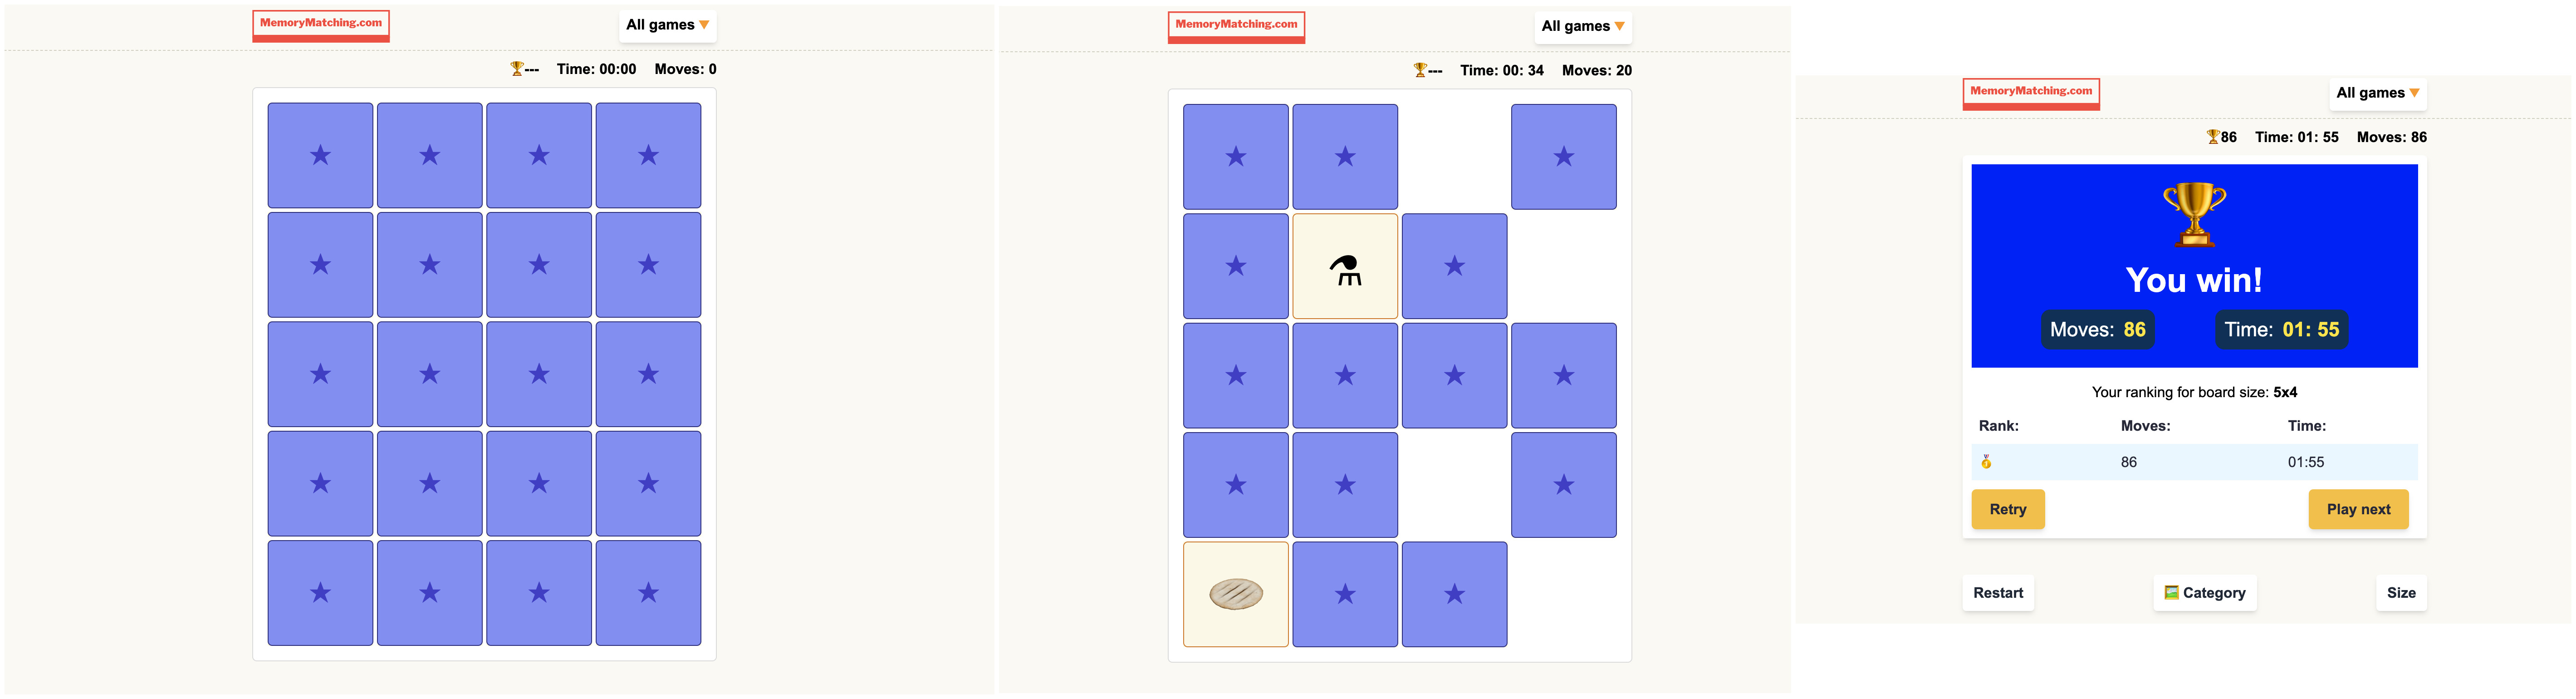
\includegraphics[width=1.0\linewidth]{dissertation/images/mem_matching.jpg}    

    \caption{Screenshots of different scenes when playing the digital card matching memory game by MemoryMatching.com
    }

    \label{fig:mem_match} 
\end{figure}

Figure \ref{fig:mem_match} shows screenshots from a digital implementation of the card-matching memory game by MemoryMatching.com. HarmonyScape will adapt this concept into a 3D space where the player-controlled character will need to make physical contact with the cards to flip them. 

\subsection{Sliding Puzzle}
A sliding puzzle is a classic game comprising a grid of square or rectangular tiles, with one space left empty to enable movement. Players aim to rearrange the tiles by sliding them horizontally or vertically into the vacant space until they align in a predetermined pattern or sequence, typically forming a complete picture or achieving a specific numerical order (Hearn, 2005).

\begin{figure}[h]
    \centering
    \begin{subfigure}[b]{0.45\textwidth}
        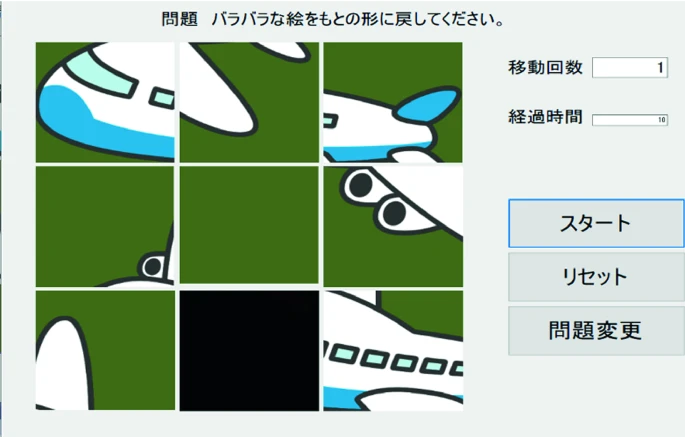
\includegraphics[width=\textwidth]{dissertation/images/uncompleted_sliding.png}
        \caption{Uncompleted sliding puzzle.}
        \label{fig:slide_uncompleted}
    \end{subfigure}
    ~ 
    \begin{subfigure}[b]{0.45\textwidth}
        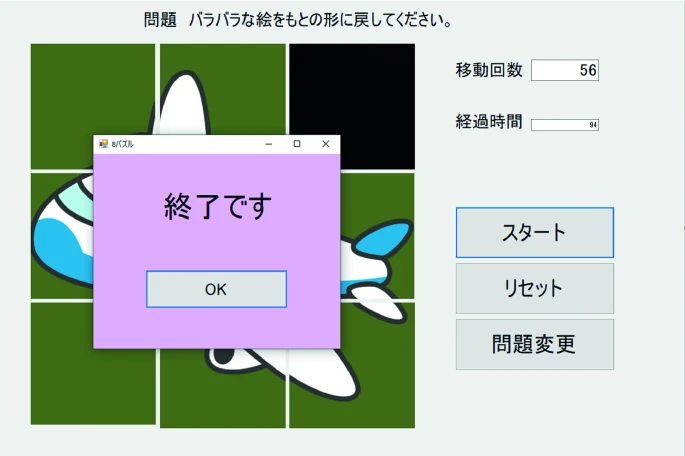
\includegraphics[width=\textwidth]{dissertation/images/completed_sliding.png}
        \caption{Completed sliding puzzle.}
        \label{fig:slide_completed}
    \end{subfigure}
    ~  
    \caption{Screenshots from a brain training application developed by Sasaki et al. (2020), demonstrating the progression of a sliding puzzle. The left image shows the puzzle before manipulation, while the right image displays the puzzle after the tiles have been rearranged to form the correct image. This example illustrates the type of sliding puzzle mechanic that HarmonyScape will also incorporate.
    }\label{fig:sliding_puzzle}
\end{figure}

Similar to the traditional sliding block puzzle and the implementation by Sasaki et al. (2020) – as illustrated in Figures \ref{fig:slide_uncompleted} and \ref{fig:slide_completed} – HarmonyScape's version challenges the user to manipulate the panels within the frame to arrange tiles into the desired order. As discussed in Section \ref{sec:sliding_dementia}, this type of puzzle engages cognitive functions – including memory, spatial awareness, and figure arrangement – that may have the potential to slow the progression of dementia (Sasaki et al., 2020).

\subsection{Music Memory Games}
The concept of memory games involving sequences of sounds can be traced back to various sources and inspirations. However, one notable origin of such games is the electronic game "Simon" which was invented by Ralph H. Baer and Howard J. Morrison and manufactured and distributed by Milton Bradley in 1978 (Baer \& Morrison, 1980). As seen in Figure \ref{fig:simon}, "Simon" consists of four colored buttons (green, red, blue, and yellow) that light up and produce unique sounds in a sequence (Baer \& Morrison, 1980). Players have to memorise the sequence and then repeat it back by pressing the corresponding buttons (Baer \& Morrison, 1980).

\begin{figure}[h]
    \centering
    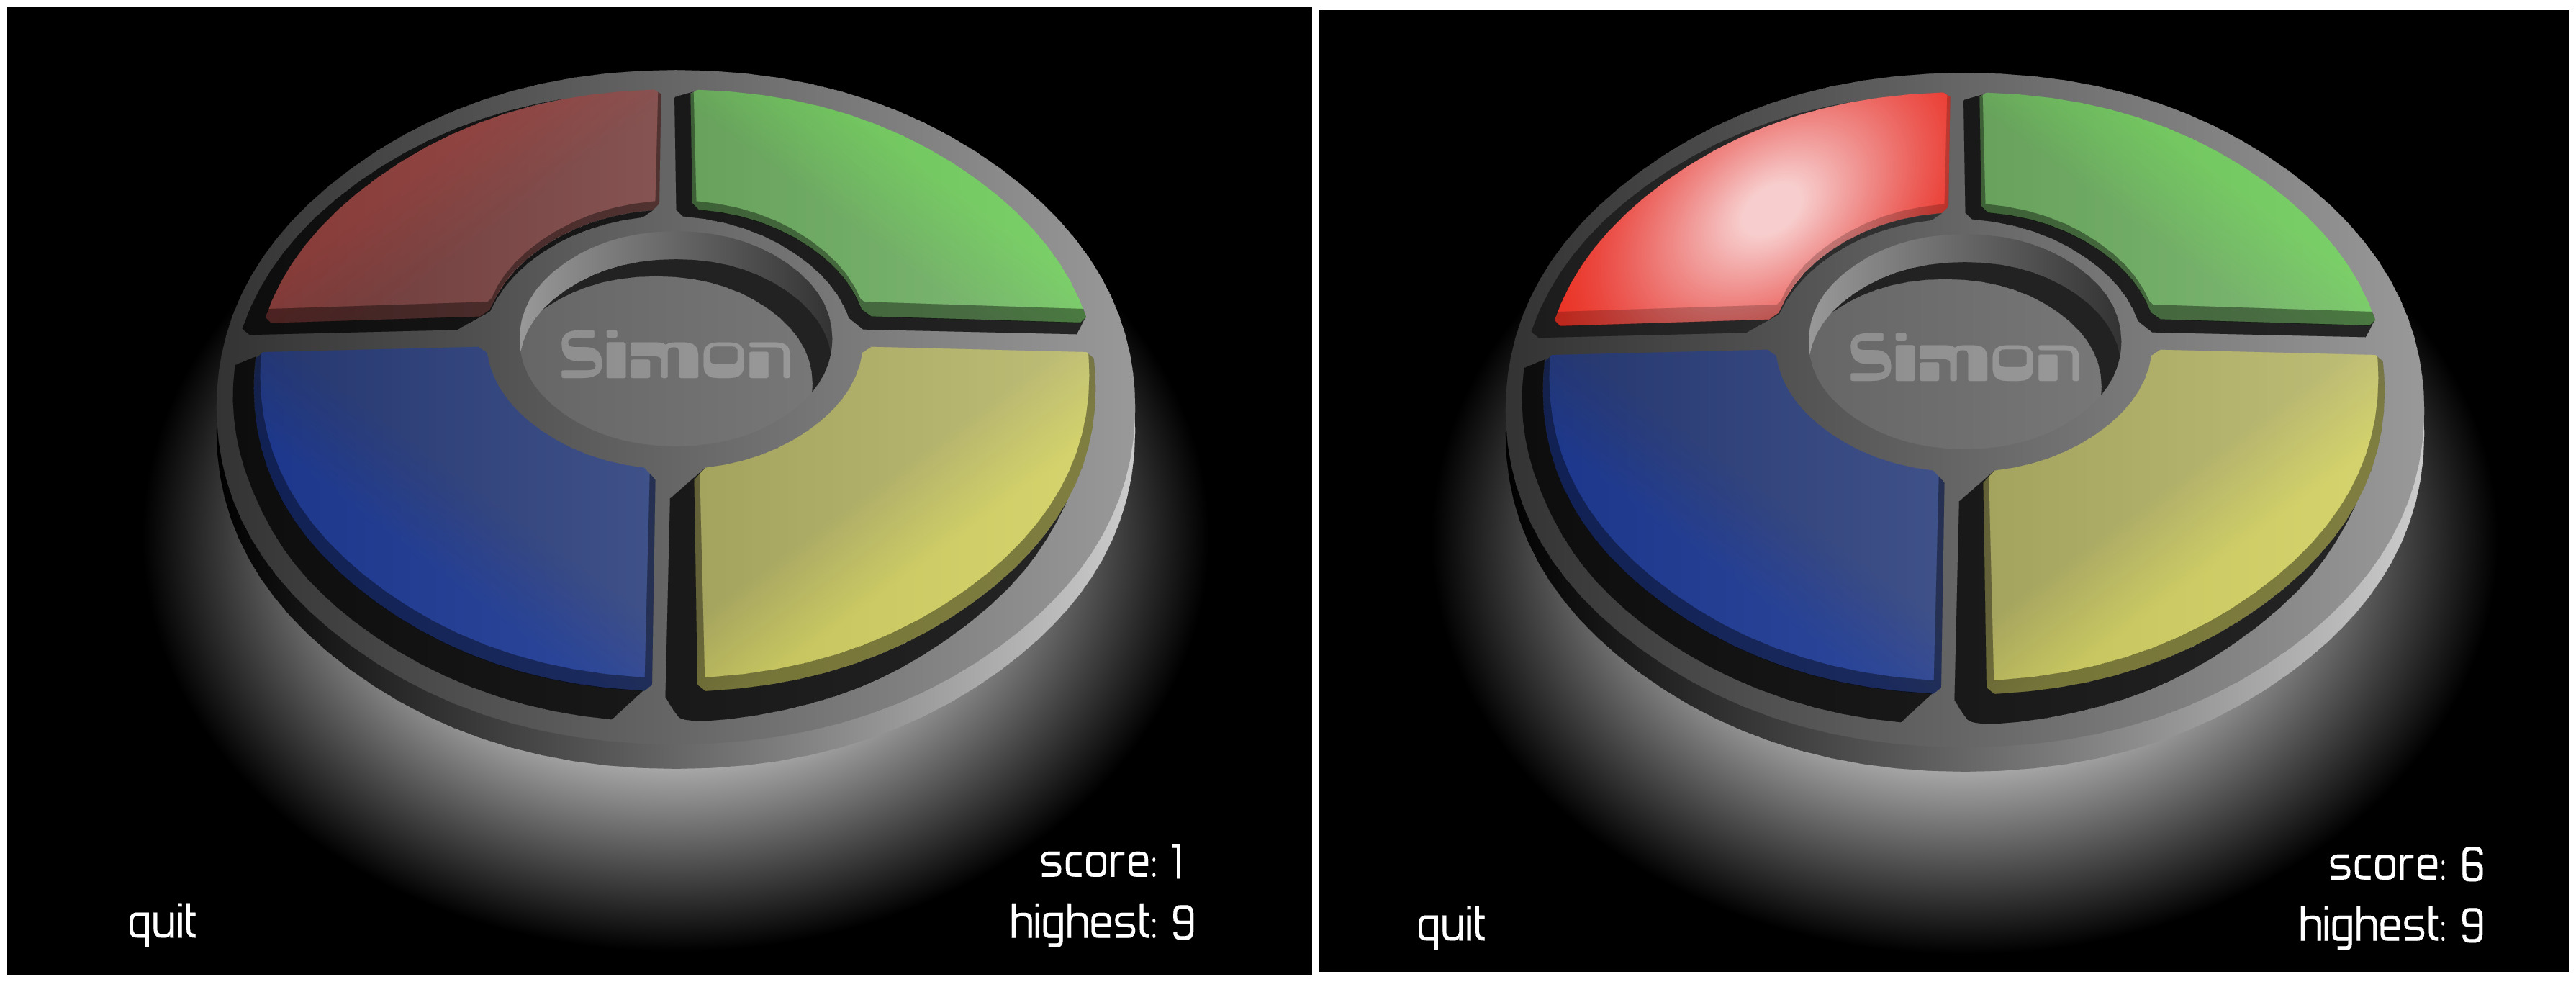
\includegraphics[width=1.0\linewidth]{dissertation/images/simon.jpg}    

    \caption{Screenshots of online implementation of the game "Simon" from "freesimon.org"
    }

    \label{fig:simon} 
\end{figure}

A systematic review conducted by Clare et al. (2003) examined the effectiveness of cognitive interventions in dementia care. The review found evidence supporting the beneficial effects of cognitive stimulation interventions on various aspects of cognitive function, including attention and concentration. Activities such as "Simon" which necessitate both selective attention to focus on specific elements and sustained attention to accurately remember and reproduce sequences, have been identified as potentially beneficial interventions for addressing the attention impairments associated with dementia, as discussed in Section \ref{sec:attention} (Clare et al., 2003).

These principles guided the design of a minigame within HarmonyScape. This minigame plays different guitar notes, requiring users to memorise the order and replicate it. Players engage with visual 'blocks' that represent unique notes, allowing them to reproduce the sequence by remembering the note order and interacting with the corresponding blocks.

The minigame's design aligns with principles of active music therapy, as detailed in Section \ref{sec:music_therapy}, where individuals engage in the process of music-making (Vink AC et al. 2004).  While the minigame isn't a therapeutic intervention in itself, it mirrors the active participation, cognitive stimulation, and sense of agency that are foundational to active music therapy approaches.

\subsection{Follow The Sound}
Games that utilise the "follow the sound" mechanic offer a unique opportunity to engage cognitive function and leverage neuroplasticity. In these games, players must navigate an environment by focusing on auditory cues, usually with the goal of locating the source of a sound. This type of gameplay directly stimulates spatial awareness and auditory processing.

The design for one of the minigames in HarmonyScape adopts a simplified approach to the follow-the-sound concept, relying exclusively on variations in volume (loudness) of the maraca sounds. This design choice, with its focus on the maracas as the primary auditory cue, creates a distinct challenge for players, requiring them to carefully analyse changes in loudness to inform their movement through the 3D environment. This gameplay mechanism emphasises volume-based spatial reasoning where players must translate changes in loudness into spatial decision-making within the virtual environment, developing a mental map based solely on auditory cues.

This stimulation of auditory perception and spatial awareness aligns with principles of neuroplasticity discussed in Section \ref{sec:neuroplasticity}. By potentially promoting the formation of new neural connections, strengthening existing pathways involved in auditory processing and spatial reasoning, and potentially improving memory and spatial awareness, this simple yet engaging game design offers a supportive and beneficial experience for individuals with dementia.

\section{Music}
HarmonyScape integrates music as a core gameplay element and a vital component of the immersive experience. This integration is realised through a unique design approach.

\subsection{Instrument Collection}
Upon successful completion of a minigame, players will discover a tangible model of the corresponding instrument available within the minigame's area. Collecting this model, accomplished through simple collision with the player -controlled character, unlocks the individual instrument track within the game's musical composition. This establishes a direct connection between player action and musical progression. Additionally, to introduce players to this concept, one instrument model will be strategically placed along the immediate path from the starting point, demonstrating this core gameplay mechanic.

\subsection{Dynamic Music Feedback}

HarmonyScape will feature an innovative dynamic music system where the tempo of the musical composition will be directly controlled by player movement.  Specifically, the tempo will respond to the character's acceleration and deceleration. When the character is stationary, the music will play at half its intended speed. As the character begins to move and accelerate, the tempo will seamlessly increase until it reaches its normal pace at the character's maximum acceleration. Conversely, as the character decelerates, the musical tempo will decrease proportionally.

It is important to note that while the music responds to the character's deceleration, the character itself will come to a complete halt when no movement input is given. This design choice prevents jarring transitions in the musical tempo, ensuring a smooth auditory experience. Whilst also avoiding any unpredictable movement that could disrupt gameplay and compromise player control. This sensitivity to potential disruption aligns with the findings in Section \ref{sec:noise_sensitivity}, which highlight the increased sensitivity to noises for individuals with dementia.

This integration of player movement directly influencing the musical experience aligns with the principles of active music therapy. By linking tempo changes to their actions, players become active participants in shaping the soundscape. This encourages physical engagement, a sense of control over the musical output, and a potentially heightened sense of accomplishment as the music reaches its full tempo through their own movement.

\section{Menu Screens}
HarmonyScape prioritises clarity and ease of use, understanding the potential challenges individuals with dementia may face. This focus aligns with the project's aim to leverage the familiarity of gaming for this generation, as discussed in the introduction. By incorporating elements like dedicated instructions, pause, title, and end screens, HarmonyScape draws inspiration from the classic video games many in this generation would have experienced. These familiar structures should provide a sense of comfort and predictability.

\subsubsection{The Title Screen} establishes a clear starting point. It will feature a simple display of the game title and a "Start" button, providing a clear entry point into the experience.

\subsubsection{The Instructions Screen} will clearly present core controls and gameplay mechanics using simple visuals and concise language. This screen acknowledges the importance of repetition and reinforcement for those with cognitive decline, creating a familiar point of reference and reducing confusion.

\subsubsection{The Pause Screen} will allow for cognitive breaks during gameplay, managing sensory input and offering moments of rest. Users will be able to easily revisit the instructions screen for reminders, supporting those who may have short-term memory difficulties.

Finally, \textbf{The End screen} offers a distinct conclusion to a gameplay session. It will include a progress summary displaying the instruments collected, reinforcing a sense of accomplishment.

\section{Progress Tracker}
HarmonyScape will incorporate a visual progress tracker to support players with keeping track of which instruments they have collected. This system features instrument icons displayed in the top left corner of the screen. Initially presented in black and white, these icons gain colour as the player successfully completes the corresponding minigame and unlocks the instrument. This colour transformation provides immediate visual feedback, signifying achievement and clearly marking which instruments have been collected.

The progress tracker's design aligns with the principles outlined in Section \ref{sec:progress_tracking} as it serves as an external memory aid, helping players with dementia to recall their progress within the game. This visual representation reinforces accomplishment as there is feedback on their progress, promoting a sense of achievement. This design aims to reduces potential frustration that might stem from memory difficulties. 

%==================================================================================================================================
\chapter{Implementation}

Chronological order of what happened, grouped by feature. For example starting with setting up the unity project, and then tackle each component in the order it was implemented.

TODO:
\begin{itemize}
    \item Terrain and Navigation:
    \begin{itemize}
        \item How the terrain was implemented (mention foliage etc.)
    \end{itemize}
    \item How each minigame was implemented:
    \begin{itemize}
        \item Card Matching
        \item Sliding Puzzle (incl. pic that shows it completed)
        \item Music Memory
        \item Follow The Sound (incl. Instructions)
        \item How the Camera Controller Script was implemented (Fixed Camera during minigames)
    \end{itemize}
    \item Dynamic Music System:
    \begin{itemize}
        \item Collection of instruments (models and triggerSFX)
        \item Audio Track Management (loading, storing instrument tracks)
        \item How the dynamic music based on movement was implemented
    \end{itemize}
    \item User Interface:
    \begin{itemize}
        \item How the Menus were implemented (Scene Loaders)
        \item Progress Tracker (Instrument Icons)
    \end{itemize}
    \item How Music Note (Guiders) were implemented
\end{itemize}

\newpage

\section{Development Environment}
This section describes the development environment that the project was set up in. This includes, Unity version, programming languages, IDEs and external libraries and assets used.

\subsection{Unity Version}
Unity Version 2022.3.10f1 LTS was chosen for the development of HarmoyScape. Unity's Long-Term Support (LTS) version was selected to ensure stability and access to extensive documentation throughout the development process.

\subsection{Programming Language}
C# is the primary language in Unity for creating custom scripts that define the behavior of game objects, handle player input, manage game logic, and interface with Unity's various systems (UI, physics, etc.). This is the sole programming language that was used in the development of HarmonyScape.

\subsection{Integrated Development Environment (IDE)}
Visual Studio Code was chosen as the development environment due to its lightweight footprint, seamless Unity integration, and robust debugging capabilities.

\subsection{External Libraries and Assets}
Music created by Ashley Garven.

\begin{itemize}
    \item TextMeshPro: \url{https://docs.unity3d.com/Manual/com.unity.textmeshpro.html}
    \item Unity-Standard-Assets: \url{https://assetstore.unity.com/packages/essentials/starter-assets-thirdperson-updates-in-new-charactercontroller-pa-196526}
    \item Rock Package: \url{https://assetstore.unity.com/packages/3d/props/exterior/rock-package-118182}
    \item Grass and Flowers Pack 1: \url{https://assetstore.unity.com/packages/2d/textures-materials/nature/grass-and-flowers-pack-1-17100}
    \item ADJ Textures: \url{https://assetstore.unity.com/packages/3d/environments/landscapes/terrain-sample-asset-pack-145808}
    \item Conifers [BOTD]: \url{https://assetstore.unity.com/packages/3d/vegetation/trees/conifers-botd-142076}
    \item RPG Monster DUO PBR Polyart: \url{https://assetstore.unity.com/packages/3d/characters/creatures/rpg-monster-duo-pbr-polyart-157762}
    \item Flooded\_Grounds: \url{https://assetstore.unity.com/packages/3d/environments/flooded-grounds-48529}
\end{itemize}

\section{Terrain and Navigation}
Before implementing any player interactivity, minigames, or the dynamic music system, we needed to create a player-controlled character. We also needed a terrain for the character to explore and interact with.

\subsection{Player-Controlled Character}
The character, originally a capsule, was originally brought in with an attached "Player Control" script, that had basic input, jump and rotation handling.

\subsubsection{HandleInput():}
The HandleInput function, within the "Player Movement Script", is responsible for gathering player input and translating it into a desired movement direction. It retrieves horizontal and vertical axis values from Unity's Input system, which correspond to the commonly used WASD and arrow keys on a keyboard, either can be used depending on player preference. Using these familiar controls promotes ease of use and minimises the learning curve for players, as discussed in \ref{sec:move_&_control}. These input values are used to construct a 3D vector (movement direction) that captures the direction the player wants to move. The magnitude of this vector is calculated and clamped between 0 and 1, ensuring that movement speed remains consistent regardless of direction. Finally, the function returns this calculated movement direction, ready to be used by the MoveAndRotatePlayer function.

\subsubsection{HandleJumping():}
The HandleJumping function, within the "Player Movement Script", manages all logic related to the player's jumping ability. It first checks if the CharacterController is grounded, meaning the player is currently touching the floor. If so, it records the current time as 'lastGroundedTime'. The function listens for the "Jump" button press (the space-bar). If pressed, the jump button pressed time is recorded. It then manages a short grace period after leaving the ground, allowing the player to jump even if they didn't press the button the exact moment they left the ground. During this grace period, it adjusts the CharacterController's step offset and sets the vertical speed (ySpeed) to initiate the jump.

\subsubsection{MoveAndRotatePlayer():}
The MoveAndRotatePlayer function, within the "Player Movement Script", takes the calculated movement direction and handles the core tasks of physically moving the player and smoothly rotating them to face their movement direction. It first creates a velocity vector by multiplying the movement direction with the player's current speed. The vertical component of this velocity (velocity.y) is set to the ySpeed variable, which is influenced by gravity and jumping. The  CharacterController 'Move' function is then called to apply this velocity, updating the player's position. Finally, if the player is moving, the function calculates a target rotation based on movement direction and smoothly rotates the player object towards that target.

\subsection{Camera System}
Cinemachine is a powerful suite of tools included within Unity that provides intelligent and dynamic camera behaviors. It simplifies the process of creating complex camera systems, allowing developers to focus on the desired look and feel of the game rather than the low-level technical implementation of camera control.

HarmonyScape implements the Cinemachine Free Look Camera, a versatile camera component designed to offer third-person style camera perspectives. This choice is rooted in the theory discussed in Section \ref{sec:third_person}, which highlights the benefits of a third-person perspective for players who may be more susceptible to simulation sickness and require enhanced situational awareness. It's commonly used in games where players need the flexibility to control the camera view to observe their surroundings and character. The Free Look Camera system consists of three virtual camera rigs (top, middle, and bottom) that orbit around a target object, with a spline system seamlessly blending between them.

In HarmonyScape, I've set the target of the Cinemachine Free Look Camera to be the player-controlled character object. This ensures that the camera remains focused on the player as they move through the game world. The Free Look Camera functions as a component of the main camera, effectively overriding Unity's standard camera controls to provide the desired dynamic camera behavior.

To prevent the camera from clipping through obstacles in the environment, I've added a Cinemachine Collider component to the Free Look Camera. This collider works in tandem with the camera system to detect potential collisions with objects in the scene. I've set the collider's strategy parameter to "Preserve Camera Distance." This means that if the camera's path would be obstructed, it smoothly readjusts its position to maintain a consistent distance from the player character, avoiding any jarring visual interruptions.

\subsubsection{How this affects the "Player Movement" script:} Within the Player Movement Script, the movement direction calculated from player input is modified based on the Cinemachine Free Look Camera's orientation. The movement direction is rotated around the vertical axis to match the camera's Y-axis rotation. This ensures that player movement aligns with the camera's view, providing an intuitive control scheme. Additionally, the movement direction is normalised to maintain consistent movement speed regardless of the applied rotation.

\section{Minigame Implementations}
The various minigames within HarmonyScape are each implemented based on the corresponding design outlined in the Design Chapter. They share a core structure, utilising a central "Minigame Master" script. This master script handles the core logic for each minigame, including tracking the player's progress, evaluating win conditions, and managing the overall flow of the minigame. The "Follow the Sound" minigame functions differently, as will be explained in the following corresponding section. 

Each minigame has its own unique set of objects placed within the game world that are specific to that minigame's functionality. These objects will often have additional scripts attached to them that manage their individual behaviours and interactions with the player.

This section will delve into the specifics of each minigame implementation, detailing the functionalities of the Minigame Master script (where applicable), the unique objects used, and any additional scripts that contribute to their functionality.

\subsection{Fixed Camera for Minigames}
Each minigame within HarmonyScape temporarily overrides the standard camera behavior whilst it is being played. This adjustment is designed to ensure that the player has a clear, unobstructed view of all the necessary minigame components. This is achieved through a dedicated "CameraController" script attached to the main camera. This script works in conjunction with trigger zones, reffred to in the scripts as "catchment areas", placed around each minigame's location.

When a player enters a minigame's catchment area, the corresponding trigger script communicates with the CameraController. The CameraController then disables the Cinemachine Brain component, taking direct control over the camera's position and rotation. The camera is repositioned and reoriented to provide an optimal view of the minigame's play area. Depending on the minigame, this might involve a top-down view or another specialised camera setup.

The player may choose to exit the catchment area before a minigame is completed if they wish to explore or attempt a different minigame. Upon exiting the minigame's catchment area, the trigger script signals the "CameraController" to reset the camera. This re-enables the Cinemachine camera, transitioning back to the free look camera used for regular exploration. Additionally, successful completion of the minigame will also disable the catchment area and reset the camera.

\subsection{Music Memory}
Completing the Music Memory minigame unlocks the Guitar part of the games soundscape. At the core of the minigame are the interactive "Note Blocks." Each Note Block is a trigger zone within the game world, and they are equipped with a NotePlayer script. This script is responsible for several key functions.

\textbf{NotePlayer Script} \newline
The NotePlayer script manages the audio playback for its associated Note Block. When the player enters the trigger area, the script plays a unique audio clip representing that block's musical note, corresponding to notes A through E on a guitar.

To provide the player with a clear indication that a note has been played, the script temporarily disables the Note Block's visual mesh and collider, making it appear to disappear, as shown in Figure \ref{fig:mem_game}. After a short delay, corresponding to the length of the audio clip, the mesh and collider are re-enabled

\begin{figure}[h]
    \centering
    \begin{subfigure}[b]{0.45\textwidth}
        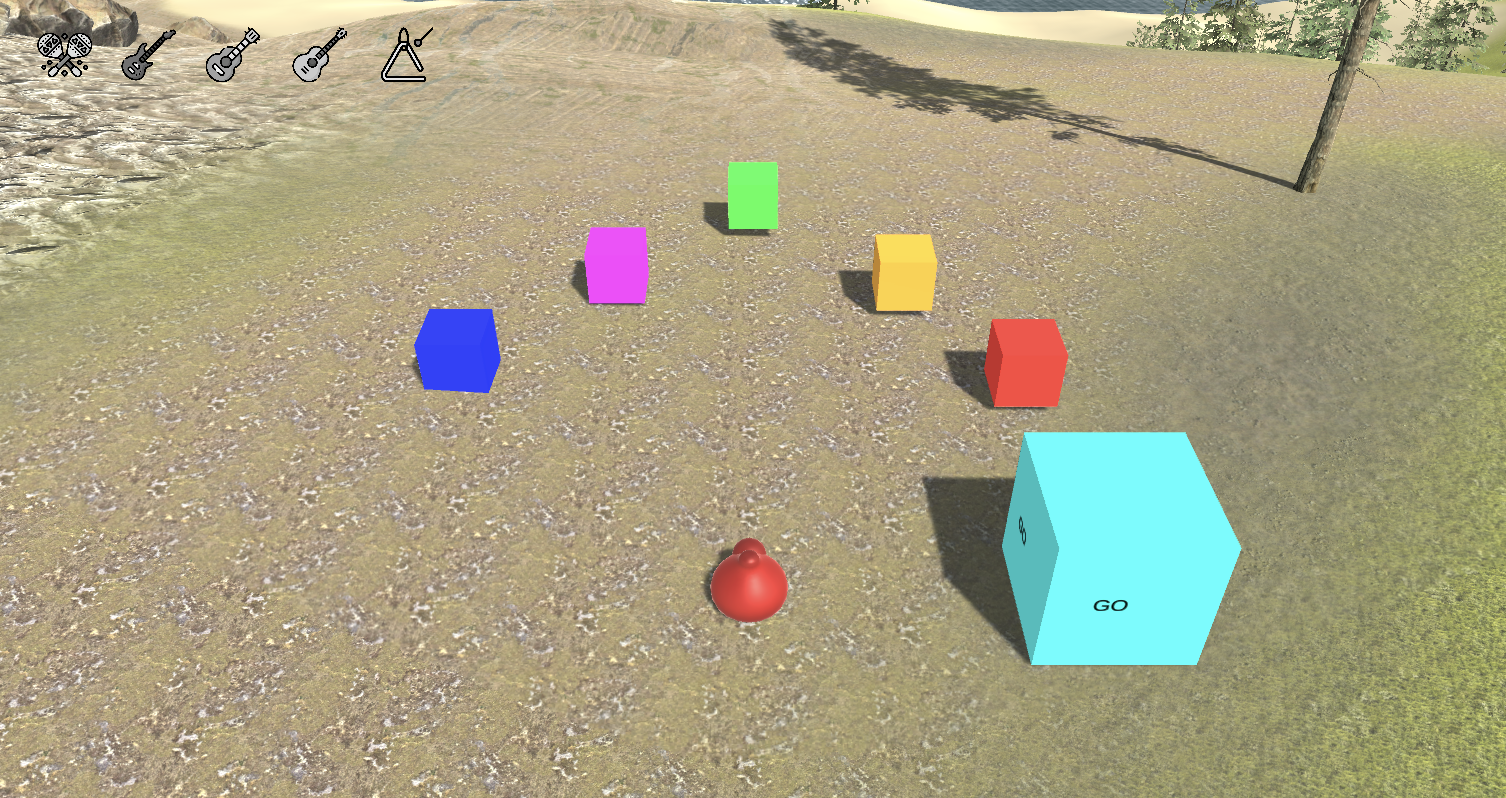
\includegraphics[width=\textwidth]{dissertation/images/Memory_Game_HarmonyScape.png}
        \caption{Whilst no note is being played during the Music Memory minigame, waiting for player to input notes.}
        \label{fig:mem_game_unplayed}
    \end{subfigure}
    ~ 
    \begin{subfigure}[b]{0.45\textwidth}
        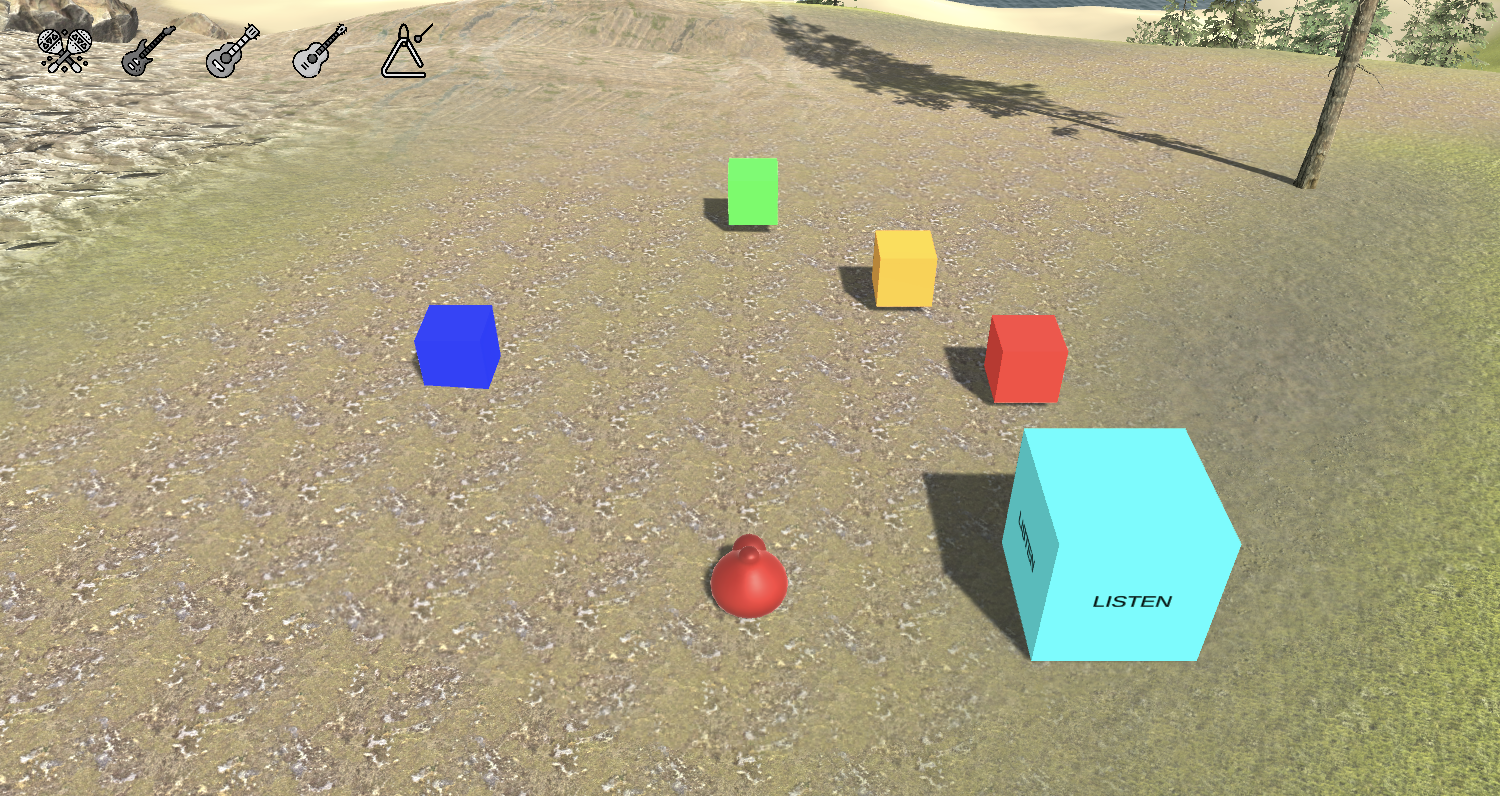
\includegraphics[width=\textwidth]{dissertation/images/Memory_Game_During.png}
        \caption{Whilst the sound corresponding to Note E is being played during the Music Memory minigame.}
        \label{fig:mem_game_played}
    \end{subfigure}
    ~     
    \caption{Note Blocks in the Music Memory minigame, demonstrating their visual transformation when a note is played.
    }
    % use the notation fig:name to cross reference a figure
    \label{fig:mem_game} 
\end{figure}

A crucial part of the NotePlayer script is its communication with the central GuitarGameMaster script, which we'll discuss later. When a Note Block is played, the script informs the GuitarGameMaster of the note type (A, B, C, D or E). This allows the GameMaster to track the player's progress within the minigame's sequence.

\textbf{GuitarGameMaster Script} \newline
The GameMaster script serves as the central script for managing the Music Memory minigame's logic, progression, and completion. It's associated with a dedicated "Start Block" in the game world, shown as the larger block in both Figures \ref{fig:mem_game_unplayed} and  \ref{fig:mem_game_played}, which triggers the minigame when the player enters its area.

This script tracks the correct sequence of notes for the minigame and the player's current progress within that sequence. It communicates with the NotePlayer scripts on each Note Block to monitor when notes are played. Upon the player entering the Start Block's trigger area, the StartGame function is activated, initialising the minigame.

During initialisation, the GameMaster prepares the minigame area by making the Note Blocks visible and enabling their colliders.  To ensure the player can focus on memorising the sequence, their movement is temporarily restricted.  The PlaySong function plays the correct sequence of notes for the player to memorise. Visual cues in the form of text changes (from "LISTEN" to "GO") signal when the player should listen for the sequence and then when they can start attempting the sequence.

The NotePlayed function is the core of progress tracking during the music memory minigame. When a Note Block's NotePlayer script informs it of a note being played, the GameMaster compares it to the expected note at the current point in the sequence. Correct notes advance the player's progress. An incorrect note will trigger the ResetGame function, resetting the sequence back to the beginning. Successfully playing all notes in the correct order triggers the FinishGame function, ending the game, removing other minigame elements, and making the guitar model available to be collected in the minigame area.

If the player needs a reminder of the note order, they can re-enter the Start Block. This will reset the currentNoteIndex and activate the PlaySong function, replaying the musical sequence. This design feature allows players to reinforce their memory of the sequence before proceeding with another attempt.


\subsection{Card Matching}
Completing the Card Matching minigame unlocks the Triangle part of the soundscapee. The core of the card-flipping minigame involves 5 pairs of cards placed within the minigame area. Each card is a cube object, with altered dimensions to resemble a card, and functions as a trigger zone.  Importantly, the cards are organized into pairs using a shared tag system (e.g., "Card\_A"). To help with identification, cards within a pair are named with a letter and number combination (e.g., "A\_1" and "A\_2"). Figure \ref{fig:card_matching_overview} provides a visual representation of the initial layout of the Card Matching minigame, with all cards face-down.

\begin{figure}[h]
  \centering
  \includegraphics[width=0.7\linewidth]{dissertation/images/CardFlip_Before.png} 

  \caption{Screenshot of the point-of-view from the player of the Card Flipping minigame area.}

  \label{fig:card_matching_overview} 
\end{figure}

\textbf{CardFlip Script} \newline
Attached to each of the cards, the CardFlip script is responsible for managing the visual flipping behaviour of individual cards and communicating these actions to the main TriangleGameMaster script, which we'll discuss in the following section. When the player collides with a card's trigger zone, the OnTriggerEnter function initiates the card-flipping process.

The FlipCard co-routine within the script handles the physical flipping animation of the card, simulating the action of flipping an actual card. It involves moving the card upwards, rotating it 180 degrees around the Z-axis, and then returning it to its original position. Importantly, the script communicates with the TriangleGameMaster via the gameMaster.FlipCard() function, informing the minigame's central logic system that a card has been flipped. There's also a FlipBack co-routine to handle flipping the cards back to their original state if the game logic requires it.

To prevent the player from interacting with multiple cards too quickly, the script manages internal state using an isFlipping flag. Additionally, it works in conjunction with the gameMaster.IsProcessingMatch() flag to ensure the game logic processes card flips avoiding multiple cards being flipped at once.

\textbf{TriangleGameMaster Script} \newline
The TriangleGameMaster script serves as the central script for managing the Card Matching minigame's logic, progression, and completion. It maintains a record of flipped cards and facilitates the primary matching logic. Upon the initiation of a card flip, the FlipCard function verifies if the card has already been flipped. If it's a new flip, the card is added to a tracking list. When two cards have been flipped over, the CheckForMatch function determines if their tags match, signifying a successful pair.

\begin{figure}[h]
  \centering
  \includegraphics[width=0.7\linewidth]{dissertation/images/CardFlip_WrongPair.png} 
  \caption{Screenshot demonstrating the `TriangleGameMaster` script's handling of incorrect card pairings. Mismatched cards are visually flipped back to their face-down state.} 
  \label{fig:card_mismatch} 
\end{figure}

If a match is found, the cards are visually deactivated to represent their removal from the active play area, as illustrated in \ref{fig:card_matching_success}. Conversely, if the cards do not match, the FlipBackCards function is called. This process, illustrated in Figure \ref{fig:card_mismatch}, restores mismatched cards to their face-down state. The AllMatchesMade function determines if all pairs have been discovered. After the player successfully pairs all card sets, the minigame ends, making the triangle model available for collection within the minigame area.

\begin{figure}[h]
  \centering
 \begin{subfigure}[t]{0.45\textwidth}
  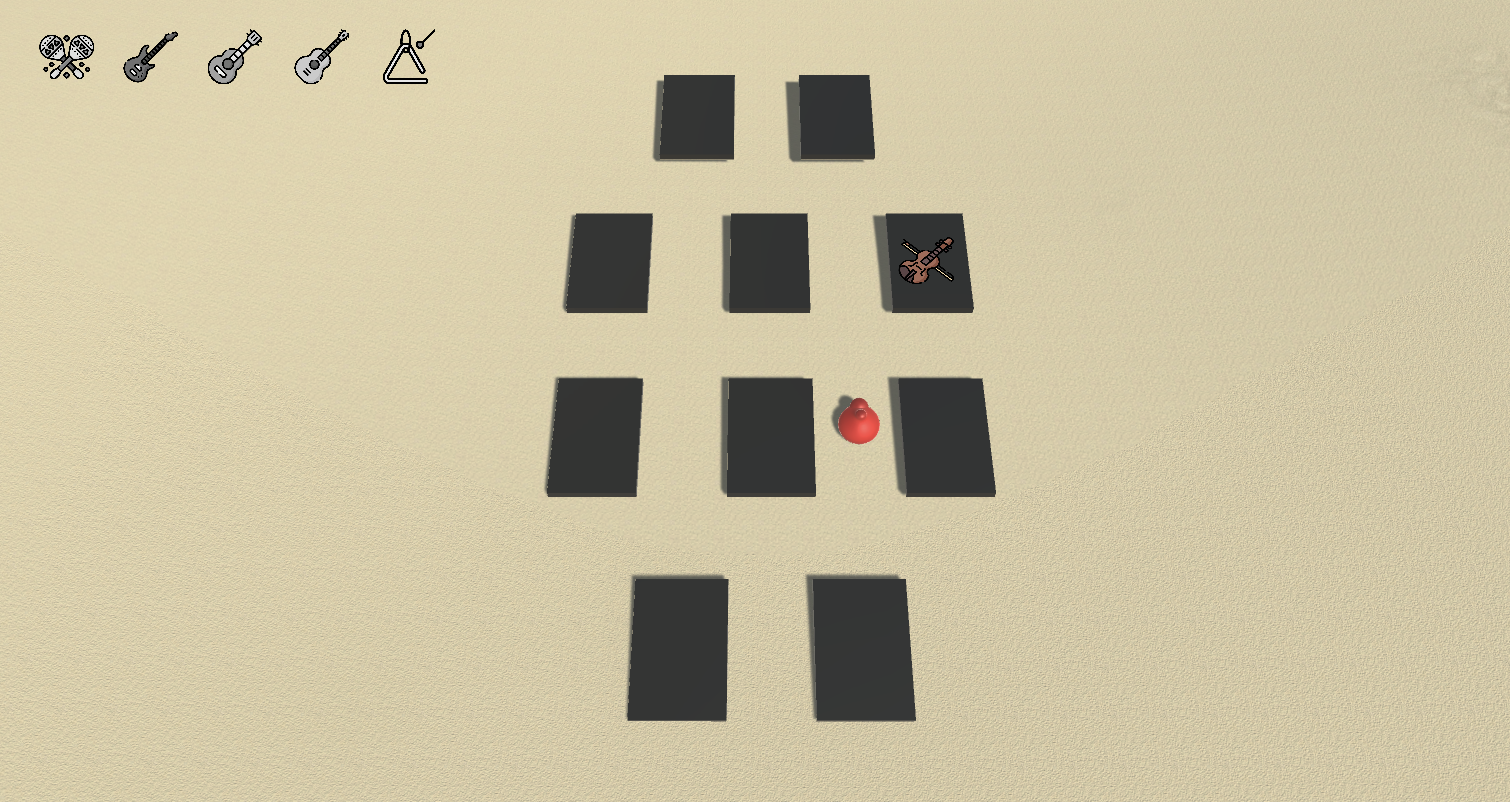
\includegraphics[width=\textwidth]{dissertation/images/CardFlip_Correct_Mid.png}
  \caption{Screenshot illustrating a successful card match as determined by the `TriangleGameMaster` script.}
  \label{fig:card_match}
 \end{subfigure}
 ~
 \begin{subfigure}[t]{0.45\textwidth}
  \includegraphics[width=\textwidth]{dissertation/images/CardFlip_Correct_After.png}
  \caption{Screenshot demonstrating the `TriangleGameMaster` script's deactivation of cards after a successful match. This represents a key step in the minigame's progression.}
  \label{fig:card_deactivation}
 \end{subfigure}  

 \caption{Series of screenshots demonstrating the visual outcomes of the `TriangleGameMaster` script's card matching logic, focusing on successful matches and their consequences.}  

 \label{fig:card_matching_success} 
\end{figure}

\subsection{Sliding Puzzle}
Series of screenshots demonstrating the visual outcomes of the `TriangleGameMaster` script's card matching logic, focusing on successful matches and their consequences.Series of screenshots demonstrating the visual outcomes of the `TriangleGameMaster` script's card matching logic, focusing on successful matches and their consequences.Series of screenshots demonstrating the visual outcomes of the `TriangleGameMaster` script's card matching logic, focusing on successful matches and their consequences.Series of screenshots demonstrating the visual outcomes of the `TriangleGameMaster` script's card matching logic, focusing on successful matches and their consequences.Series of screenshots demonstrating the visual outcomes of the `TriangleGameMaster` script's card matching logic, focusing on successful matches and their consequences.Series of screenshots demonstrating the visual outcomes of the `TriangleGameMaster` script's card matching logic, focusing on successful matches and their consequences.Series of screenshots demonstrating the visual outcomes of the `TriangleGameMaster` script's card matching logic, focusing on successful matches and their consequences.

% \begin{figure}[h]
%   \centering
%   \includegraphics[width=0.7\linewidth]{dissertation/images/CardFlip_Correct_Before.png} 

%   \caption{Screenshot illustrating the card-flipping animation controlled by the CardFlip script. The card has transitioned from its face-down state to its face-up state.}

%   \label{fig:card_flip_in_action} 
% \end{figure}

\subsection{Follow The Sound}
...

% What did you do to implement this idea, and what technical achievements did you make?
% \section{Guidance}
% You can't talk about everything. Cover the high level first, then cover important, relevant or impressive details.



% \section{General points}

% These points apply to the whole dissertation, not just this chapter.



% \subsection{Figures}
% \emph{Always} refer to figures included, like Figure \ref{fig:relu}, in the body of the text. Include full, explanatory captions and make sure the figures look good on the page.
% You may include multiple figures in one float, as in Figure \ref{fig:synthetic}, using \texttt{subcaption}, which is enabled in the template.



% % Figures are important. Use them well.
% \begin{figure}
%     \centering
%     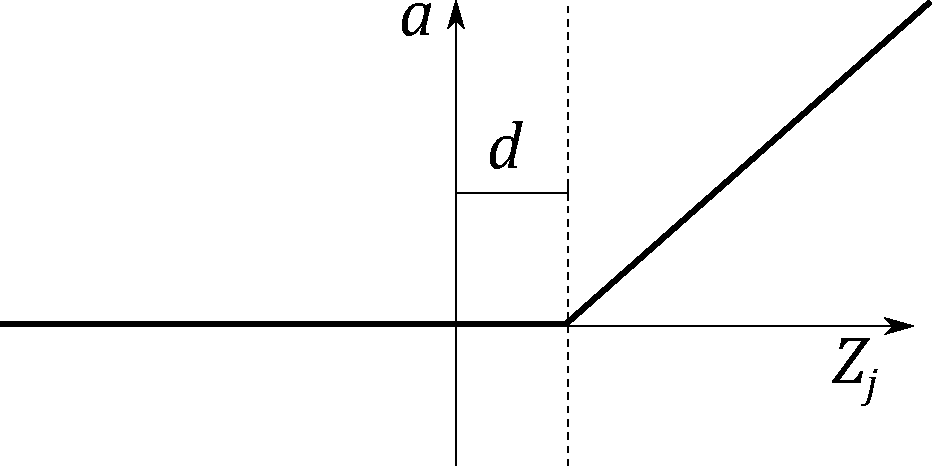
\includegraphics[width=0.5\linewidth]{images/relu.pdf}    

%     \caption{In figure captions, explain what the reader is looking at: ``A schematic of the rectifying linear unit, where $a$ is the output amplitude,
%     $d$ is a configurable dead-zone, and $Z_j$ is the input signal'', as well as why the reader is looking at this: 
%     ``It is notable that there is no activation \emph{at all} below 0, which explains our initial results.'' 
%     \textbf{Use vector image formats (.pdf) where possible}. Size figures appropriately, and do not make them over-large or too small to read.
%     }

%     % use the notation fig:name to cross reference a figure
%     \label{fig:relu} 
% \end{figure}


% \begin{figure}
%     \centering
%     \begin{subfigure}[b]{0.45\textwidth}
%         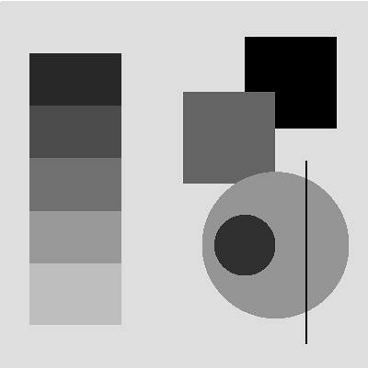
\includegraphics[width=\textwidth]{images/synthetic.png}
%         \caption{Synthetic image, black on white.}
%         \label{fig:syn1}
%     \end{subfigure}
%     ~ %add desired spacing between images, e. g. ~, \quad, \qquad, \hfill etc. 
%       %(or a blank line to force the subfigure onto a new line)
%     \begin{subfigure}[b]{0.45\textwidth}
%         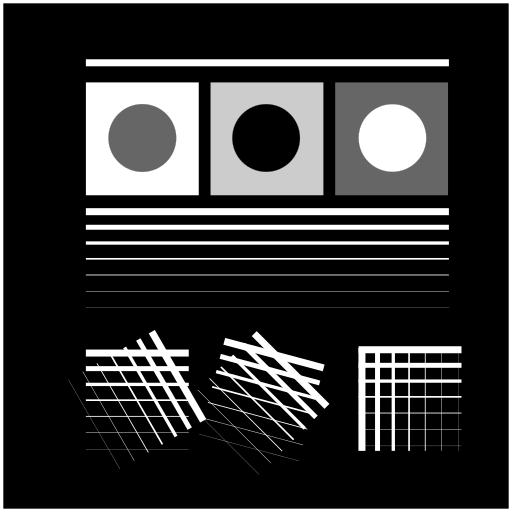
\includegraphics[width=\textwidth]{images/synthetic_2.png}
%         \caption{Synthetic image, white on black.}
%         \label{fig:syn2}
%     \end{subfigure}
%     ~ %add desired spacing between images, e. g. ~, \quad, \qquad, \hfill etc. 
%     %(or a blank line to force the subfigure onto a new line)    
%     \caption{Synthetic test images for edge detection algorithms. \subref{fig:syn1} shows various gray levels that require an adaptive algorithm. \subref{fig:syn2}
%     shows more challenging edge detection tests that have crossing lines. Fusing these into full segments typically requires algorithms like the Hough transform.
%     This is an example of using subfigures, with \texttt{subref}s in the caption.
%     }\label{fig:synthetic}
% \end{figure}

% \clearpage

% \subsection{Equations}

% Equations should be typeset correctly and precisely. Make sure you get parenthesis sizing correct, and punctuate equations correctly 
% (the comma is important and goes \textit{inside} the equation block). Explain any symbols used clearly if not defined earlier. 

% For example, we might define:
% \begin{equation}
%     \hat{f}(\xi) = \frac{1}{2}\left[ \int_{-\infty}^{\infty} f(x) e^{2\pi i x \xi} \right],
% \end{equation}    
% where $\hat{f}(\xi)$ is the Fourier transform of the time domain signal $f(x)$.

% \subsection{Algorithms}
% Algorithms can be set using \texttt{algorithm2e}, as in Algorithm \ref{alg:metropolis}.

% % NOTE: line ends are denoted by \; in algorithm2e
% \begin{algorithm}
%     \DontPrintSemicolon
%     \KwData{$f_X(x)$, a probability density function returing the density at $x$.\; $\sigma$ a standard deviation specifying the spread of the proposal distribution.\;
%     $x_0$, an initial starting condition.}
%     \KwResult{$s=[x_1, x_2, \dots, x_n]$, $n$ samples approximately drawn from a distribution with PDF $f_X(x)$.}
%     \Begin{
%         $s \longleftarrow []$\;
%         $p \longleftarrow f_X(x)$\;
%         $i \longleftarrow 0$\;
%         \While{$i < n$}
%         {
%             $x^\prime \longleftarrow \mathcal{N}(x, \sigma^2)$\;
%             $p^\prime \longleftarrow f_X(x^\prime)$\;
%             $a \longleftarrow \frac{p^\prime}{p}$\;
%             $r \longleftarrow U(0,1)$\;
%             \If{$r<a$}
%             {
%                 $x \longleftarrow x^\prime$\;
%                 $p \longleftarrow f_X(x)$\;
%                 $i \longleftarrow i+1$\;
%                 append $x$ to $s$\;
%             }
%         }
%     }
    
% \caption{The Metropolis-Hastings MCMC algorithm for drawing samples from arbitrary probability distributions, 
% specialised for normal proposal distributions $q(x^\prime|x) = \mathcal{N}(x, \sigma^2)$. The symmetry of the normal distribution means the acceptance rule takes the simplified form.}\label{alg:metropolis}
% \end{algorithm}

% \subsection{Tables}

% If you need to include tables, like Table \ref{tab:operators}, use a tool like https://www.tablesgenerator.com/ to generate the table as it is
% extremely tedious otherwise. 

% \begin{table}[]
%     \caption{The standard table of operators in Python, along with their functional equivalents from the \texttt{operator} package. Note that table
%     captions go above the table, not below. Do not add additional rules/lines to tables. }\label{tab:operators}
%     %\tt 
%     \rowcolors{2}{}{gray!3}
%     \begin{tabular}{@{}lll@{}}
%     %\toprule
%     \textbf{Operation}    & \textbf{Syntax}                & \textbf{Function}                            \\ %\midrule % optional rule for header
%     Addition              & \texttt{a + b}                          & \texttt{add(a, b)}                                    \\
%     Concatenation         & \texttt{seq1 + seq2}                    & \texttt{concat(seq1, seq2)}                           \\
%     Containment Test      & \texttt{obj in seq}                     & \texttt{contains(seq, obj)}                           \\
%     Division              & \texttt{a / b}                          & \texttt{div(a, b) }  \\
%     Division              & \texttt{a / b}                          & \texttt{truediv(a, b) } \\
%     Division              & \texttt{a // b}                         & \texttt{floordiv(a, b)}                               \\
%     Bitwise And           & \texttt{a \& b}                         & \texttt{and\_(a, b)}                                  \\
%     Bitwise Exclusive Or  & \texttt{a \textasciicircum b}           & \texttt{xor(a, b)}                                    \\
%     Bitwise Inversion     & \texttt{$\sim$a}                        & \texttt{invert(a)}                                    \\
%     Bitwise Or            & \texttt{a | b}                          & \texttt{or\_(a, b)}                                   \\
%     Exponentiation        & \texttt{a ** b}                         & \texttt{pow(a, b)}                                    \\
%     Identity              & \texttt{a is b}                         & \texttt{is\_(a, b)}                                   \\
%     Identity              & \texttt{a is not b}                     & \texttt{is\_not(a, b)}                                \\
%     Indexed Assignment    & \texttt{obj{[}k{]} = v}                 & \texttt{setitem(obj, k, v)}                           \\
%     Indexed Deletion      & \texttt{del obj{[}k{]}}                 & \texttt{delitem(obj, k)}                              \\
%     Indexing              & \texttt{obj{[}k{]}}                     & \texttt{getitem(obj, k)}                              \\
%     Left Shift            & \texttt{a \textless{}\textless b}       & \texttt{lshift(a, b)}                                 \\
%     Modulo                & \texttt{a \% b}                         & \texttt{mod(a, b)}                                    \\
%     Multiplication        & \texttt{a * b}                          & \texttt{mul(a, b)}                                    \\
%     Negation (Arithmetic) & \texttt{- a}                            & \texttt{neg(a)}                                       \\
%     Negation (Logical)    & \texttt{not a}                          & \texttt{not\_(a)}                                     \\
%     Positive              & \texttt{+ a}                            & \texttt{pos(a)}                                       \\
%     Right Shift           & \texttt{a \textgreater{}\textgreater b} & \texttt{rshift(a, b)}                                 \\
%     Sequence Repetition   & \texttt{seq * i}                        & \texttt{repeat(seq, i)}                               \\
%     Slice Assignment      & \texttt{seq{[}i:j{]} = values}          & \texttt{setitem(seq, slice(i, j), values)}            \\
%     Slice Deletion        & \texttt{del seq{[}i:j{]}}               & \texttt{delitem(seq, slice(i, j))}                    \\
%     Slicing               & \texttt{seq{[}i:j{]}}                   & \texttt{getitem(seq, slice(i, j))}                    \\
%     String Formatting     & \texttt{s \% obj}                       & \texttt{mod(s, obj)}                                  \\
%     Subtraction           & \texttt{a - b}                          & \texttt{sub(a, b)}                                    \\
%     Truth Test            & \texttt{obj}                            & \texttt{truth(obj)}                                   \\
%     Ordering              & \texttt{a \textless b}                  & \texttt{lt(a, b)}                                     \\
%     Ordering              & \texttt{a \textless{}= b}               & \texttt{le(a, b)}                                     \\
%     % \bottomrule
%     \end{tabular}
%     \end{table}
% \subsection{Code}

% Avoid putting large blocks of code in the report (more than a page in one block, for example). Use syntax highlighting if possible, as in Listing \ref{lst:callahan}.

% \begin{lstlisting}[language=python, float, caption={The algorithm for packing the $3\times 3$ outer-totalistic binary CA successor rule into a 
%     $16\times 16\times 16\times 16$ 4 bit lookup table, running an equivalent, notionally 16-state $2\times 2$ CA.}, label=lst:callahan]
%     def create_callahan_table(rule="b3s23"):
%         """Generate the lookup table for the cells."""        
%         s_table = np.zeros((16, 16, 16, 16), dtype=np.uint8)
%         birth, survive = parse_rule(rule)

%         # generate all 16 bit strings
%         for iv in range(65536):
%             bv = [(iv >> z) & 1 for z in range(16)]
%             a, b, c, d, e, f, g, h, i, j, k, l, m, n, o, p = bv

%             # compute next state of the inner 2x2
%             nw = apply_rule(f, a, b, c, e, g, i, j, k)
%             ne = apply_rule(g, b, c, d, f, h, j, k, l)
%             sw = apply_rule(j, e, f, g, i, k, m, n, o)
%             se = apply_rule(k, f, g, h, j, l, n, o, p)

%             # compute the index of this 4x4
%             nw_code = a | (b << 1) | (e << 2) | (f << 3)
%             ne_code = c | (d << 1) | (g << 2) | (h << 3)
%             sw_code = i | (j << 1) | (m << 2) | (n << 3)
%             se_code = k | (l << 1) | (o << 2) | (p << 3)

%             # compute the state for the 2x2
%             next_code = nw | (ne << 1) | (sw << 2) | (se << 3)

%             # get the 4x4 index, and write into the table
%             s_table[nw_code, ne_code, sw_code, se_code] = next_code

%         return s_table

% \end{lstlisting}

%==================================================================================================================================
\chapter{Evaluation} 

TODOO:
\begin{itemize}
    \item Summarise based on results in user study
    \item Future work could implement directional sound in Follow The Sound mini game
\end{itemize}

How good is your solution? How well did you solve the general problem, and what evidence do you have to support that?

\section{Guidance}
\begin{itemize}
    \item
        Ask specific questions that address the general problem.
    \item
        Answer them with precise evidence (graphs, numbers, statistical
        analysis, qualitative analysis).
    \item
        Be fair and be scientific.
    \item
        The key thing is to show that you know how to evaluate your work, not
        that your work is the most amazing product ever.
\end{itemize}

% \section{Evidence}
% Make sure you present your evidence well. Use appropriate visualisations, reporting techniques and statistical analysis, as appropriate.

% If you visualise, follow the basic rules, as illustrated in Figure \ref{fig:boxplot}:
% \begin{itemize}
% \item Label everything correctly (axis, title, units).
% \item Caption thoroughly.
% \item Reference in text.
% \item \textbf{Include appropriate display of uncertainty (e.g. error bars, Box plot)}
% \item Minimize clutter.
% \end{itemize}

% See the file \texttt{guide\_to\_visualising.pdf} for further information and guidance.

% \begin{figure}
%     \centering
%     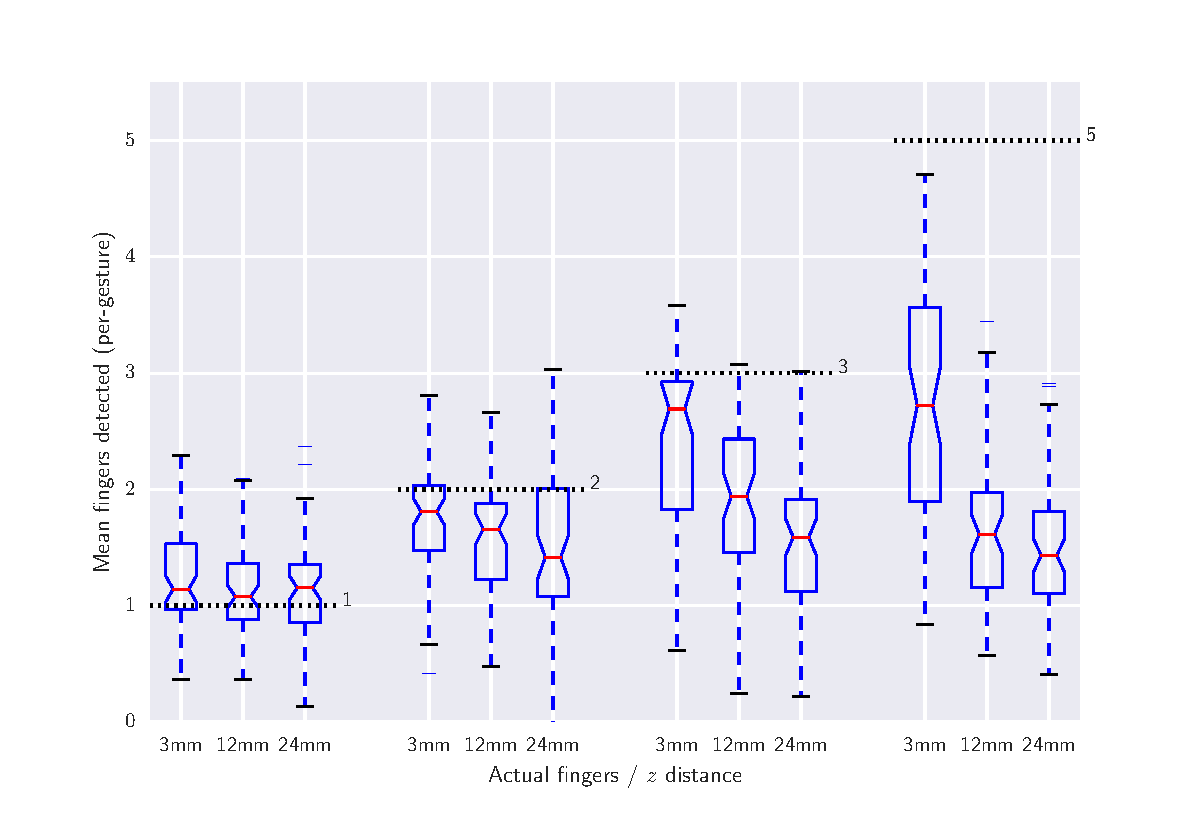
\includegraphics[width=1.0\linewidth]{images/boxplot_finger_distance.pdf}    

%     \caption{Average number of fingers detected by the touch sensor at different heights above the surface, averaged over all gestures. Dashed lines indicate
%     the true number of fingers present. The Box plots include bootstrapped uncertainty notches for the median. It is clear that the device is biased toward 
%     undercounting fingers, particularly at higher $z$ distances.
%     }

%     % use the notation fig:name to cross reference a figure
%     \label{fig:boxplot} 
% \end{figure}


%==================================================================================================================================
\chapter{Conclusion}    
Summarise the whole project for a lazy reader who didn't read the rest (e.g. a prize-awarding committee).
\section{Guidance}
\begin{itemize}
    \item
        Summarise briefly and fairly.
    \item
        You should be addressing the general problem you introduced in the
        Introduction.        
    \item
        Include summary of concrete results (``the new compiler ran 2x
        faster'')
    \item
        Indicate what future work could be done, but remember: \textbf{you
        won't get credit for things you haven't done}.
\end{itemize}

%==================================================================================================================================
%
% 
%==================================================================================================================================
%  APPENDICES  

\begin{appendices}

\chapter{Appendices}

Typical inclusions in the appendices are:

\begin{itemize}
\item
  Copies of ethics approvals (required if obtained)
\item
  Copies of questionnaires etc. used to gather data from subjects.
\item
  Extensive tables or figures that are too bulky to fit in the main body of
  the report, particularly ones that are repetitive and summarised in the body.

\item Outline of the source code (e.g. directory structure), or other architecture documentation like class diagrams.

\item User manuals, and any guides to starting/running the software.

\end{itemize}

\textbf{Don't include your source code in the appendices}. It will be
submitted separately.

\end{appendices}

%==================================================================================================================================
%   BIBLIOGRAPHY   

% The bibliography style is abbrvnat
% The bibliography always appears last, after the appendices.

\bibliographystyle{abbrvnat}

\bibliography{l4proj}

\end{document}
